%============================================
\subsection{Dark Matter Halo Merger Trees}
%============================================

%============================================
\subsubsection{Terminology}
%============================================

Before having a closer look at dark matter halo merger trees and how to make them, some clear definitions and terminology on the subject are necessary.
In this work, the terminology as set by the Merger Tree Comparison Project \parencite{SUSSING_COMPARISON} is adapted:

\begin{itemize}
	\item A \emph{halo} is a dark-matter condensation as returned by a halo-finder.
	
	\item Haloes may be spatially nested: in that case the outer halo is the \emph{main halo} and the other haloes are	\emph{subhaloes}.
		Where no distinction between subhaloes and main haloes is made, they will be collectively referred to as \emph{clumps}.
	
	\item Haloes are defined at distinct {\emph snapshots}. 
		Snapshots correspond to	particular values of cosmic time and contain the particle IDs, mass, location \& velocity for each dark matter particle in the simulation.  
	
	\item For two snapshots at different times to the older one (i.e. higher redshift) is referred to as $A$ and the younger one (i.e. lower redshift) as $B$.
	
	\item A \emph{graph} is a set of ordered halo pairs, $(H_A,H_B)$, where $H_A$ is older than $H_B$. 
		It is the purpose of the merger-tree codes to produce a graph that best represents the growth of structure over cosmic time.
		$H_A$ and $H_B$ are usually taken from adjacent snapshots, but this is not a requirement as there are occasions where haloes lose their identity and then reappear at a later time.
	
	\item Recursively, $H_A$ itself and progenitors of $H_A$ are \emph{progenitors} of $H_B$.
		Where it is necessary to distinguish $H_A$ from earlier progenitors, the term \emph{direct progenitor} will be used.
	
	\item Recursively, $H_B$ itself and descendants of $H_B$ are \emph{descendants} of $H_A$.  
		Where it is necessary to distinguish $H_B$ from later descendants, the term \emph{direct descendant} will be used.
	
	\item This work is primarily concerned with \emph{merger trees} for
	which there is \emph{precisely one direct descendant for every halo}. 
		Note that it is possible for haloes near the minimum mass limit to have zero descendants: such haloes are omitted from the analysis.
	
	\item In the case that there are multiple direct progenitors, it is required that precisely one of these is labelled the \emph{ main progenitor}.
	
	\item The \emph{main branch} of a halo is a complete list of main progenitors tracing back along its cosmic history.
	
\end{itemize}








%============================================
\subsubsection{Aim}
%============================================

\begin{figure}[p]
    \centering
    %---------------------
    % Horizontal
    %---------------------
%    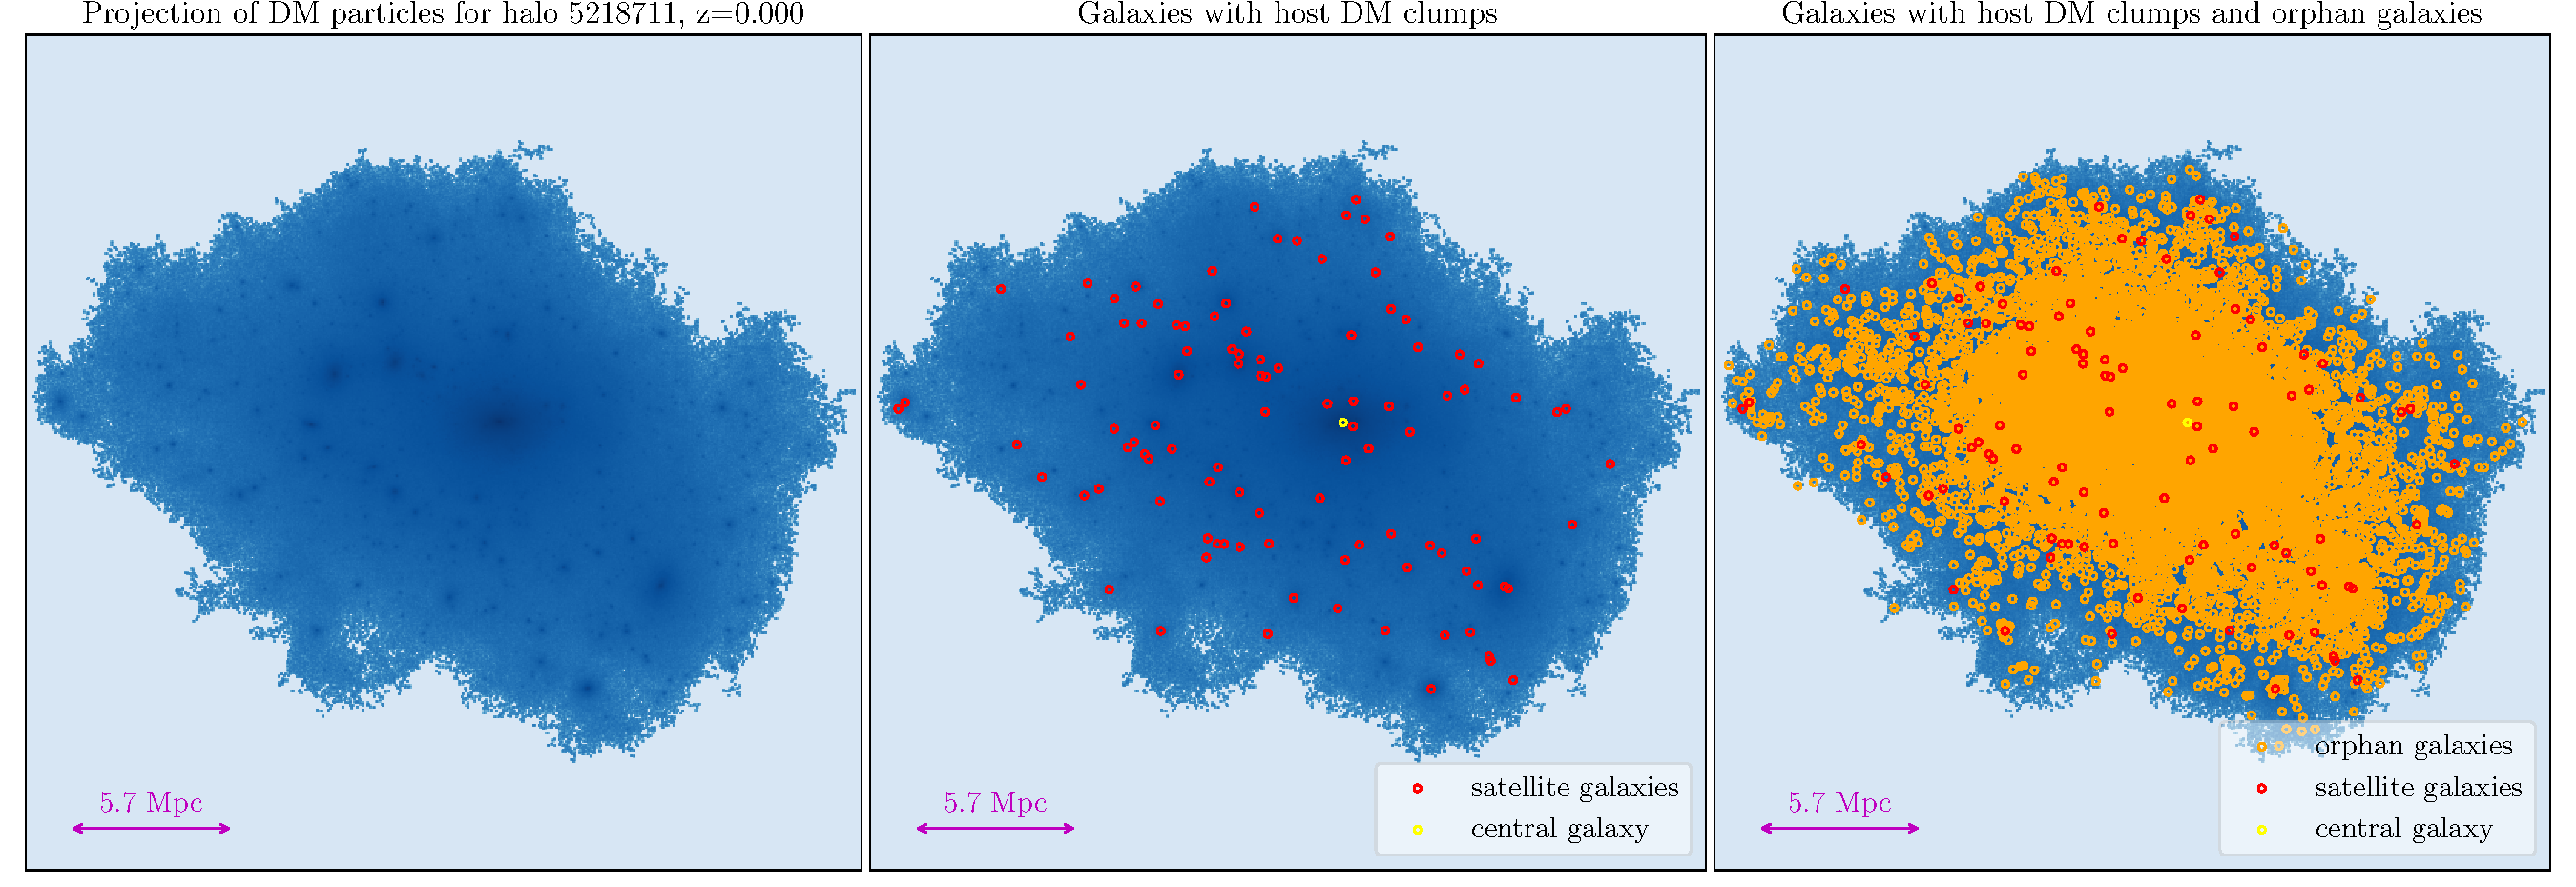
\includegraphics[width=\textwidth]{./images/galaxies/69MPC/halostats_image_output_00041-halo-5218711.pdf}
%    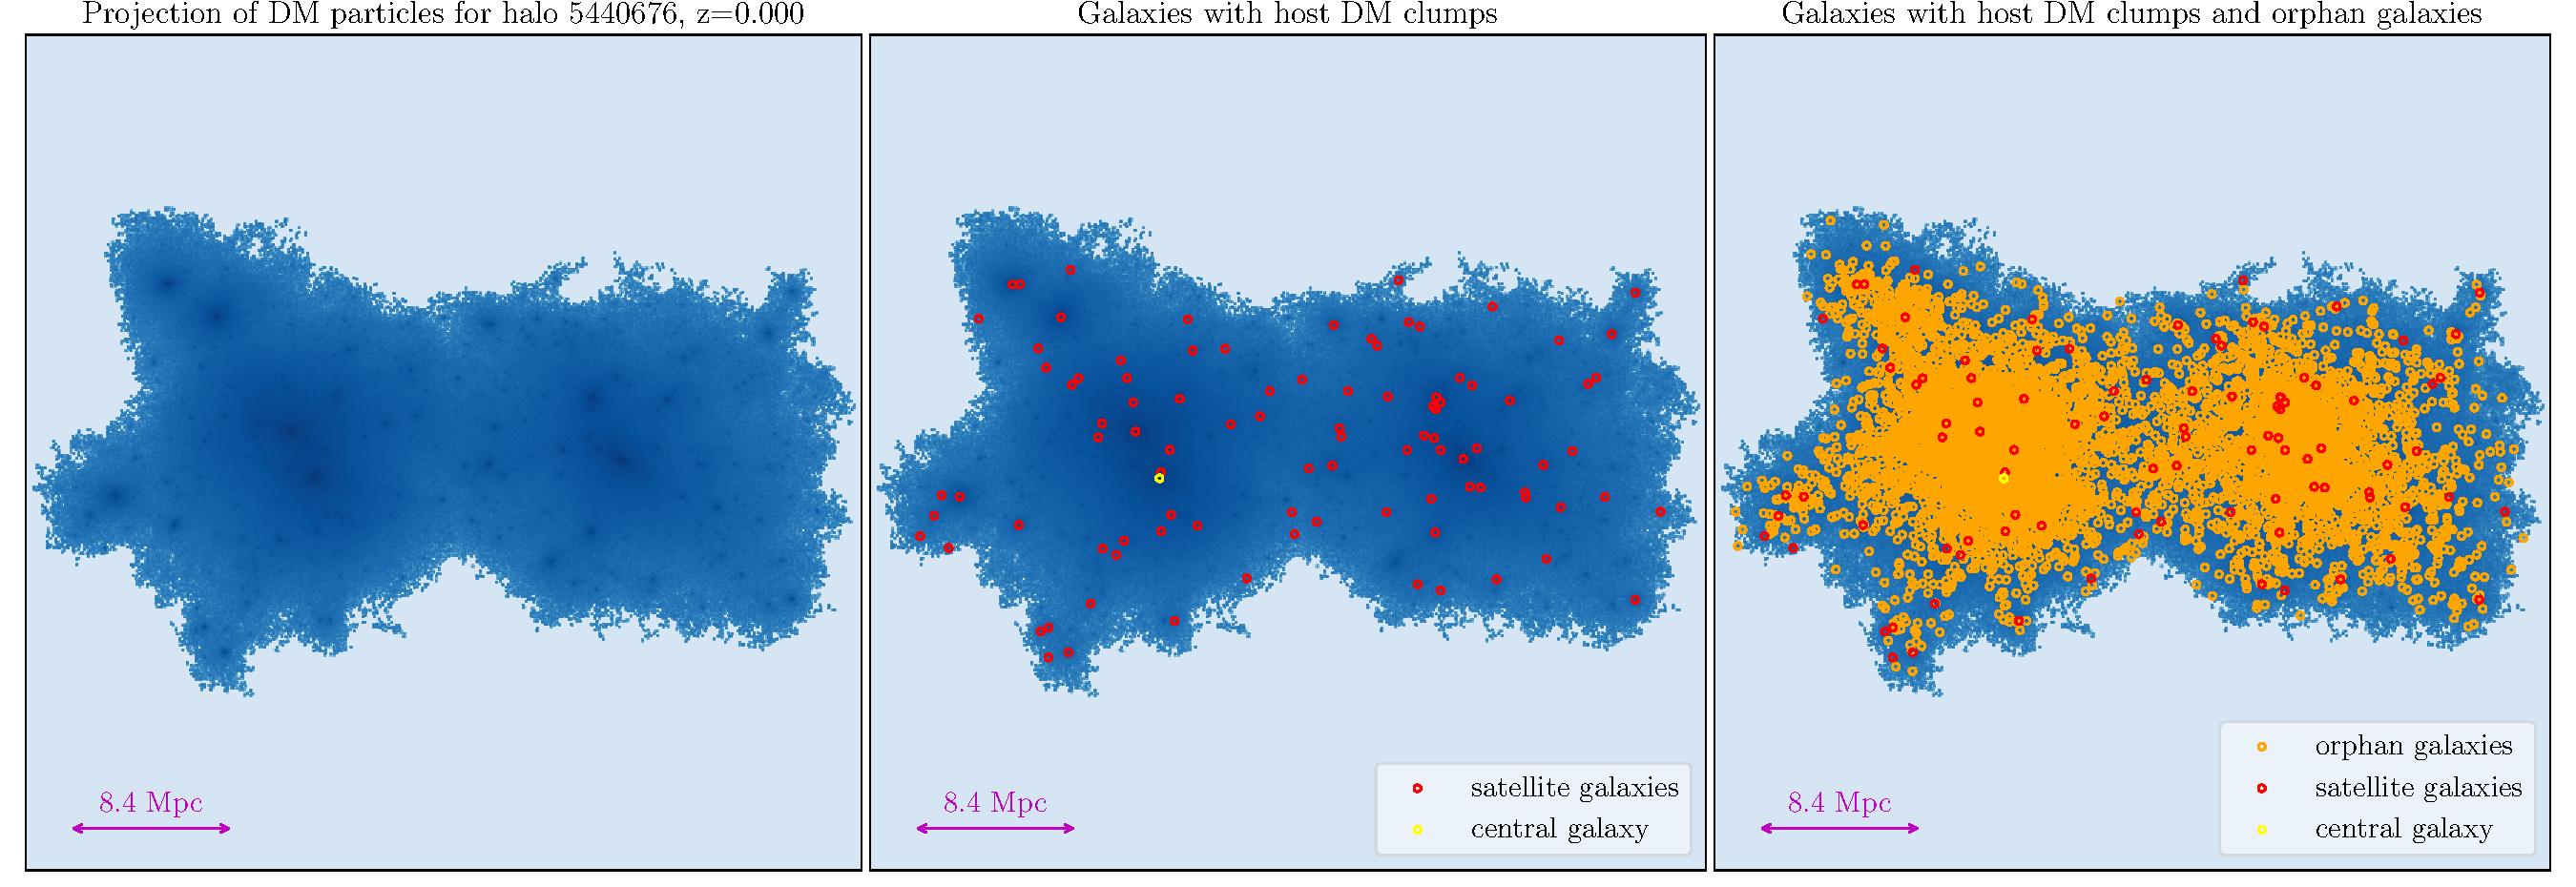
\includegraphics[width=\textwidth]{./images/galaxies/100MPC/halostats_image_output_00041-halo-5440676.pdf}
    %---------------------
    % Vertical
    %---------------------
    \minipage[t]{.43\textwidth}
        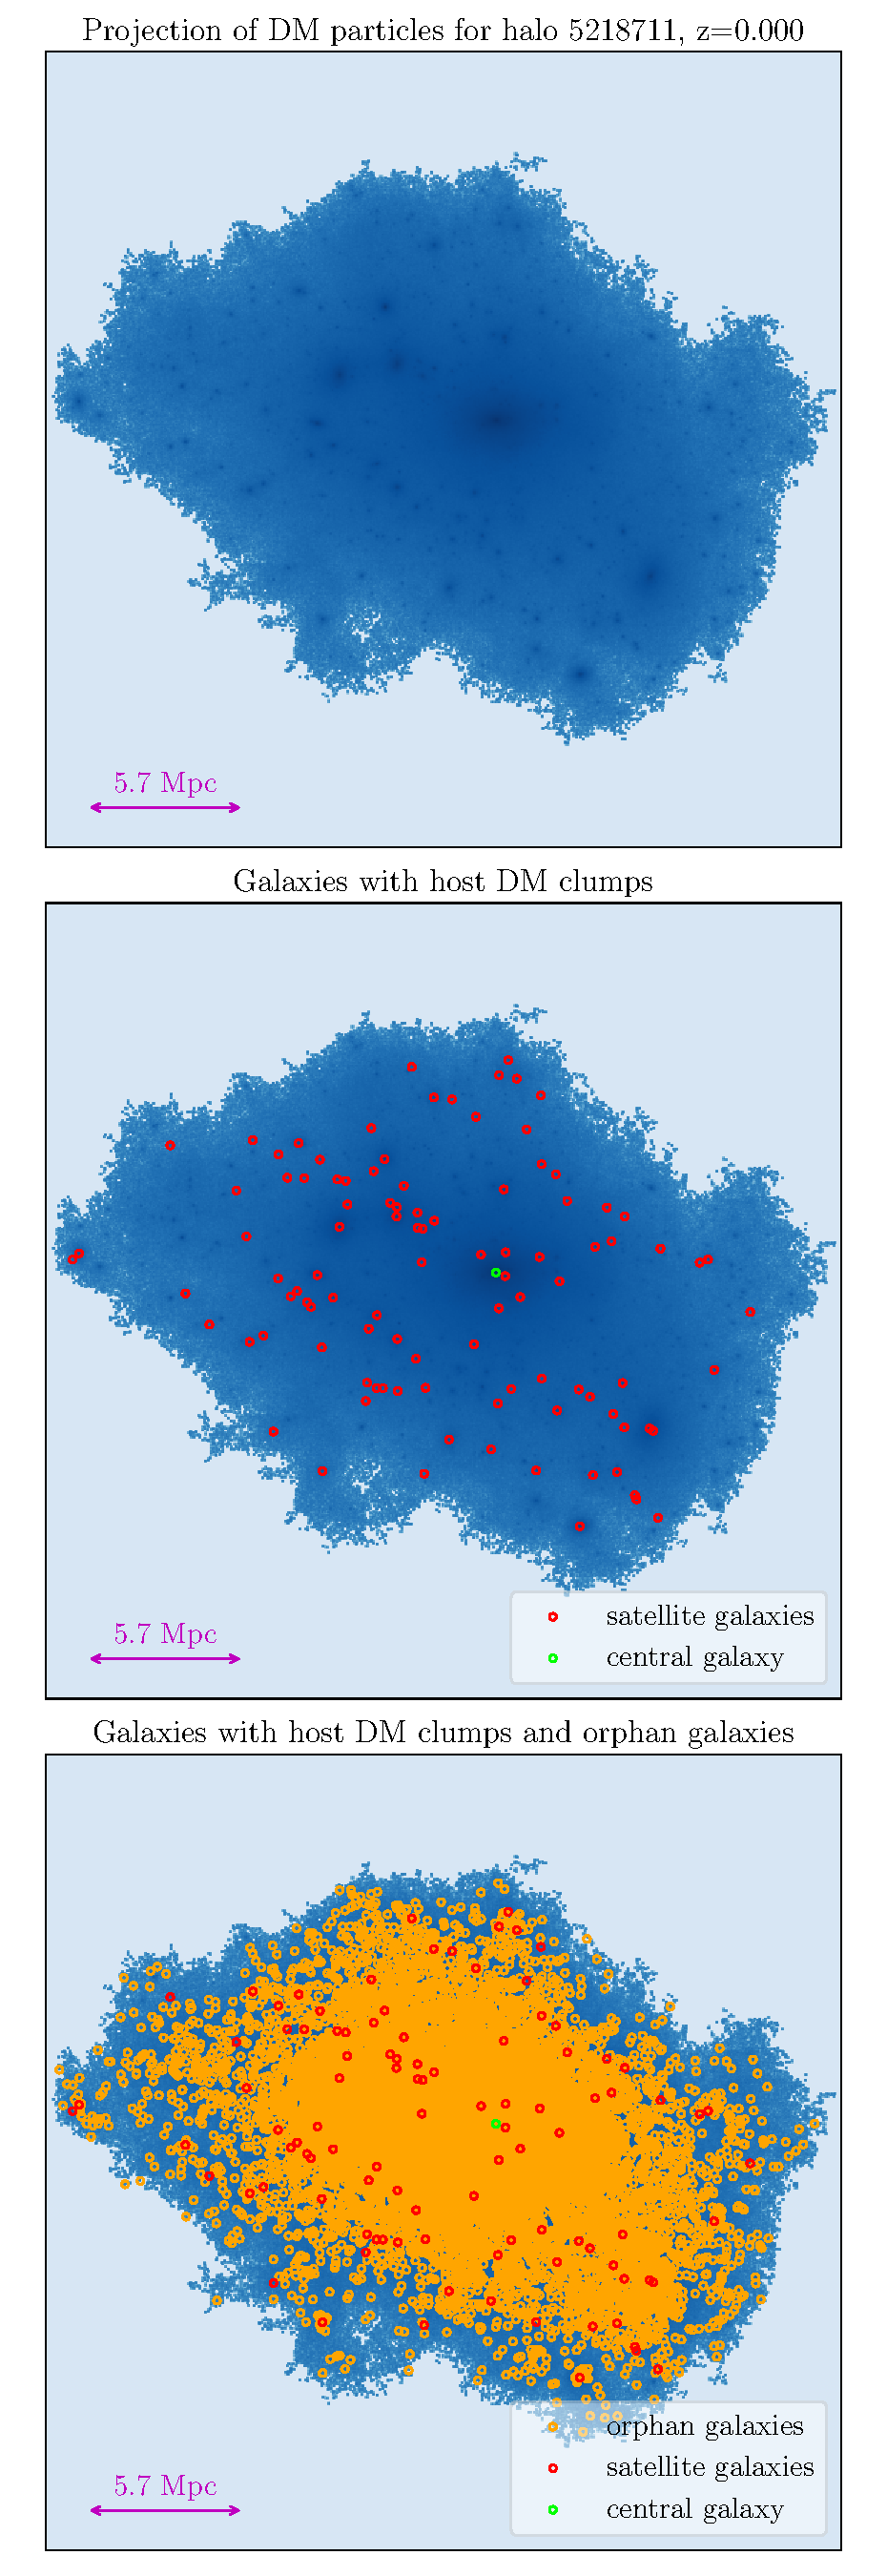
\includegraphics[width=\textwidth]{./images/galaxies/69MPC/vertical-halostats_image_output_00041-halo-5218711.pdf}
    \endminipage
    \hspace*{\fill}
    \minipage[t]{.43\textwidth}
        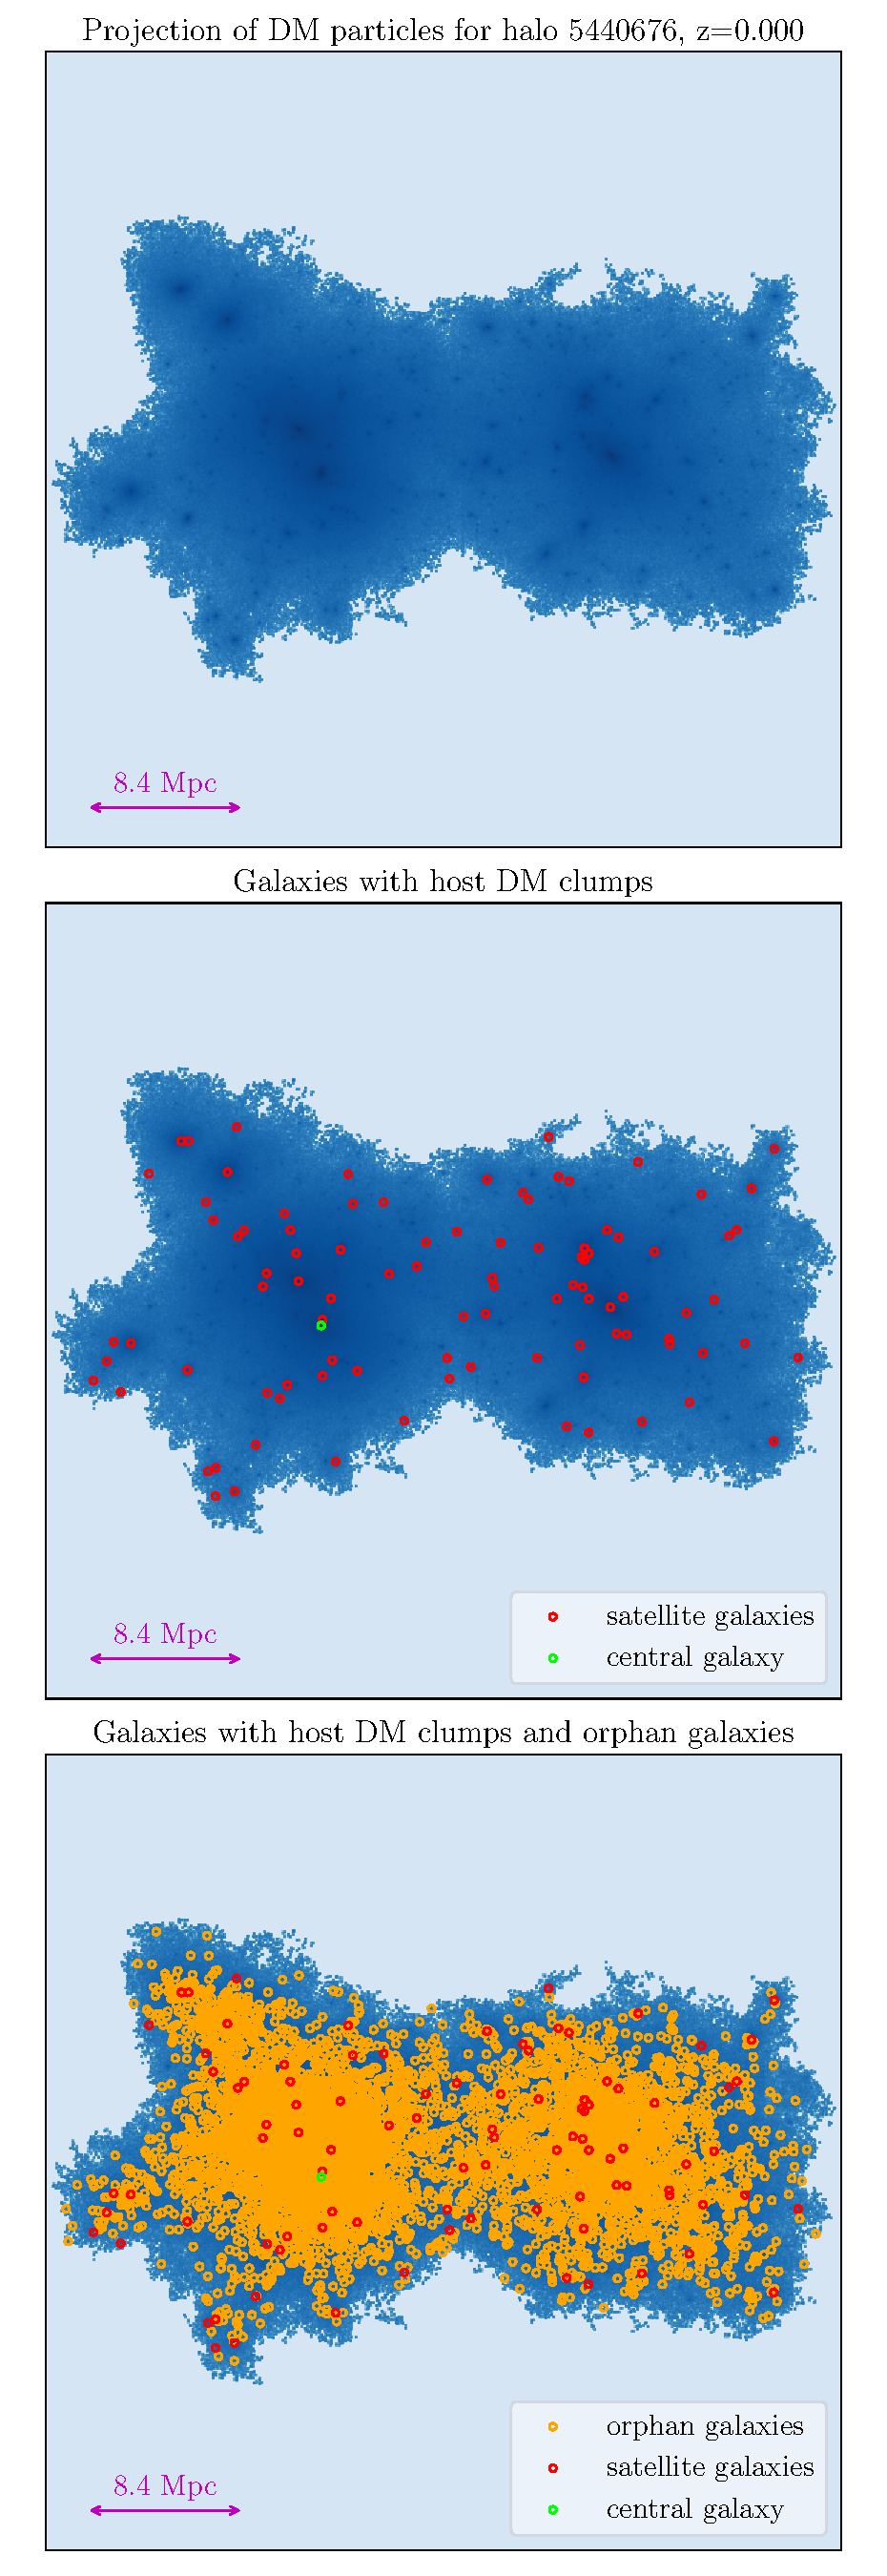
\includegraphics[width=\textwidth]{./images/galaxies/100MPC/vertical-halostats_image_output_00041-halo-5440676.pdf}
    \endminipage
    \caption{Projection along the $z$-axis of the most massive dark matter haloes from the \gsmall\ (left) and the \glarge\ (right)
        simulations with marked galaxy positions at $z=0$.
        The simulations used are described in section \ref{chap:sim_galaxy}.
        The circles representing galaxies do not indicate their physical size.
        The arrows indicating the physical lenght of the image correspond to one fifth of the plotted region in each direction.\\
        Noticeably, some dark matter condensations appear to have no satellite galaxy assigned to them.
        There are two reasons for this: Firstly, because the visualisation technique used is a projection, no information on how stretched along the $z$-axis these clumps are is shown.
        Secondly, the stricter unbinding criterion was applied for these simulations, where a particle is only considered bound if it can't escape the spatial boundaries of the clump (see section \ref{chap:unbinding} for details).
        This tends to remove more particles from a clump then when not applied, and possibly remove enough particles from a clump so that it doesn't satisfy a lower mass threshold condition.
        If that is the case, such clumps are removed from the (sub)halo catalogue.
    }
    \label{fig:galaxies_in_halo}
\end{figure}


Merger trees follow the growth and merges of dark matter haloes over cosmic history.
In the hierarchical structure formation scenario, starting with a nearly uniform density field of the Universe, large, massive haloes are thought to form mainly through a series of merging events of smaller haloes over cosmic time.
Figure \ref{fig:mergertree_scheme} shows schematically how a massive halo may form through consecutive merging events.
Because galaxies form inside the potential well dark matter haloes, knowledge of how many merging events a halo underwent during its lifetime is crucial for accurate mock galaxy catalogues.
After a merging event, the galaxy of the smaller halo that has been ``swallowed up'' by a bigger one has no reason to simply vanish without a trace. 
The ``swallowed up'' halo might become a subhalo, or, if it is small enough or after some time, it might not be detectable as substructure in the simulation any more.
Galaxies of haloes that dissolve in this manner are referred to as ``\emph{orphan galaxies}''.
Their importance can be clearly seen in figure \ref{fig:galaxies_in_halo}, which shows the most massive haloes resulting from two cosmological simulations described in section \ref{chap:sim_galaxy}.
If orphan galaxies are taken into account, the number of galaxies in these haloes grows from less than 100 galaxies based on subhaloes with a minimal number of bound particles to a few thousand.


\begin{figure}[H]
    \centering
    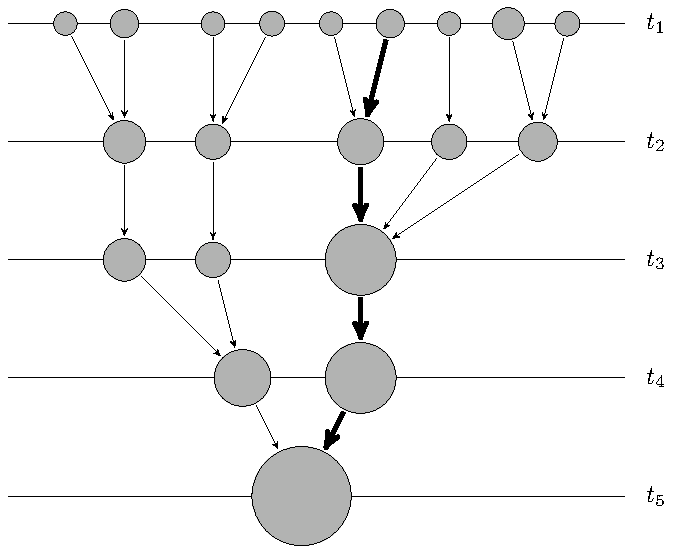
\includegraphics[width=.5\textwidth]{./images/tikz/mergertree.pdf}
    \caption{Illustration of a merger tree, showing the formation history of some halo over cosmic time through a series of merging events with $t_1 < t_2 < t_3 < t_4 < t_5$. 
        The $x$-axis has no physical meaning.
        The main branch of this merger tree is signified by the thicker arrows.
        The size of the circles represents the haloes' masses.}
    \label{fig:mergertree_scheme}
\end{figure}


In dark matter simulations haloes however are only defined at distinct snapshots.
The aim of a merger tree code is to link haloes from an earlier snapshot to the haloes of the consecutive snapshot, i.e. to find the descendants of the haloes of the earlier snapshot within the consecutive snapshot, thus enabling the tracking of growth and merges of haloes in a simulation.

A straightforward method to link progenitors with descendants in adjacent snapshots is to trace particles by their unique ID.
All but one merger tree algorithm tested in \cite{SUSSING_COMPARISON} also rely on particle IDs to connect progenitor clumps with descendant ones.
Essentially this would mean to check in which clumps of a later snapshot $B$ did particles that were found to be in a clump in an earlier snaphot $A$ end up in.
Other methods are also conceivable: \texttt{JMERGE} \parencite{SUSSING_COMPARISON} for example uses the properties of haloes at both snapshot $A$ and $B$ to estimate where each halo should be at the midpoint in time between the two snapshots, and then links the haloes based on these calculated positions.

Finally, the presented merger tree algorithm is required to run on the fly and in parallel using the MPI library.










%==========================================================
\subsubsection{Restrictions, Complications and Solutions}
%==========================================================

To obtain a merger tree, as opposed to a merger graph, each progenitor may have exactly one direct descendant halo. 
Descendants however may have multiple direct progenitors. 
In this case, exactly one of the direct progenitors must be labelled as the main progenitor.
The other direct progenitors of this descendant are then assumed to have merged into the main direct progenitor to form the descendant.

Descendant candidates for any progenitor are identified by tracing particles of that progenitor across snapshots.
Naturally, those particles may end up in multiple clumps, giving multiple descendant candidates for a progenitor.
In such cases, the most promising descendant candidate will be called the \emph{main descendant}.
To find a main progenitor and a main descendant, usually some merit function $\mathcal{M}$ is defined, which is to be maximised or minimised, depending on its definition.

Let $\mathcal{M}_{pd,adj}(A,B_i)$ be the merit function to be maximised for a number of descendants $B_i$ to be a main descendant of a progenitor $A$, and let $n_{mb}$ be the total number of particles of progenitor $A$ that are being traced to a later adjacent snapshot, where the descendants $B_i$ are found.
$n_{mb}$ may or may not be the total number of particles of $A$. 
Then a straightforward ansatz for $\mathcal{M}_{pd,adj}(A,B_i)$ would be:
\begin{equation}
    \mathcal{M}_{pd,adj}(A,B) \propto \frac{n_{A \cap B_i}}{n_{mb}}
\end{equation}
where $n_{A \cap B_i}$ is the number of traced particles of $A$ found in $B$.
Similarly, if $\mathcal{M}_{dp,adj}(A_i,B)$ is the merit function to be maximised for a number of progenitors $A_i$ to be the main progenitor of a descendant $B$ in an adjacent snapshot, then a straightforward ansatz would be:
\begin{equation}
    \mathcal{M}_{dp,adj}(A_i,B) \propto \frac{n_{A_i \cap B}}{N_B}
\end{equation}
where $N_B$ is the total number of particles in clump $B$.
In these two merit functions, $n_{mb}$ and $N_B$ constitute a norm.

These two merit functions can be united into one by considering that when evaluating the value of $\mathcal{M}_{adj}$, in both cases the denominator is independent of the candidates for which it is evaluated:
The number of particles traced, $n_{mb}$, won't depend on what or how many descendant candidates have been identified.
The same goes for total the number of particles of clump $B$, which won't change by choosing some progenitor candidate or the other as the main progenitor.
So the merit function for adjacent snapshots can be reduced to
\begin{equation}
    \mathcal{M}_{adj}(A,B) \propto n_{A \cap B}
\end{equation}





A complication arises from the fact that the clump-finder in \ramses\ defines the main halo as the one with the highest density peak.
If for example a halo consists of two similar clumps with similar height of their respective density peaks, then it is possible that over time small variations in the density peak will lead to oscillations in the identification of the main halo between these two clumps.
The particle unbinding algorithm will then look for unbound particles in what was found to be the subhalo and pass them on to the main halo, increasing its mass and decreasing the subhalo's mass.
This is amplified when a particle is defined to be bound if and only if it mustn't cross the spatial boundaries of the subhalo.
Therefore, if between snapshots the identification of which clump is the main halo varies, then strong mass oscillations can be expected.
To counter this behaviour, the merit function can be extended to prefer candidates with similar masses:
\begin{equation}
    \mathcal{M}_{adj}(A,B) = \frac{n_{A \cap B}}{\frac{m_>}{m_<}-1} \label{eq:merit}
\end{equation}
The factor $(m_>/m_< - 1) ^{-1}$ increases as $m_> \rightarrow m_<$, where $m_<$ and $m_>$ are the smaller and larger mass of the descendant-progenitor pair $(A,B)$, respectively.
An overview of what merit functions were chosen in other merger tree algorithms is given in table 1 in \cite{SUSSING_COMPARISON}.



\begin{figure}[H]
    \centering
    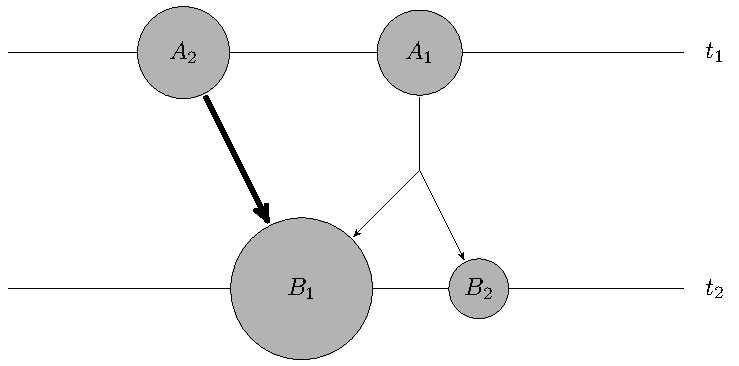
\includegraphics[width=.5\textwidth]{./images/tikz/fracture.pdf}
    \caption{Illustration of a progenitor $A_1$ at time $t_1$ which is partially merged into a descendant $B_1$ at time $t_2 > t_1$, but some other part $B_2$ isn't. 
        Because $A_1$ is not the main progenitor of $B_1$, by assigning its descendant only according to the merit function \eqref{eq:merit} would not pass on its formation history to $B_2$, but treat it as newly formed.
        The size of the circles represents the haloes' masses, the $x$-axis has no physical meaning.
        }
    \label{fig:fracture}
\end{figure}



Since a descendant may have multiple progenitors, but each progenitor may have only one descendant, a question that needs to be adressed is how to deal with situations where multiple descendant candidates, i.e. descendant clumps that contain tracked particles of some progenitor, are found.
Problems arise for example when some progenitor $A_1$ is not the main progenitor of its main descendant $B_1$, but also has fractured into another descendant candidate $B_2$.
This situation is schematically shown in figure \ref{fig:fracture}.
Relying only on the merit function \eqref{eq:merit}, progenitor $A_1$ will seem to have merged with $A_2$, the direct progenitor of $B_1$, in order to form $B_1$.
The fractured remainder, $B_2$, will be treated as newly formed, provided it has no other progenitor candidates.
In this case the entire formation history of $B_2$ would be lost.
In order to preserve history, instead of merging progenitor $A_1$ into $B_1$, the link to $B_2$ should be preferred.
This is simpler to implement into the algorithm than to express via the merit function.
If $A_1$ is not the main progenitor of its main descendant $B_2$, then don't merge it into $B_2$ until all of $A_1$'s descendant candidates have found their own main progenitor, and give priority to $A_1$ for being a progenitor to some descendant which is not its main descendant over merging it into its main descendant.












Finally, in some cases a subhalo passing close to the core of its main halo may not be identified as an individual subhalo and appear to be ``swallowed up'' by the main halo, but will re-emerge at a later snapshot.
Such a scenario is shown in figure \ref{fig:jumper-demo}.
When this occurs, the merger tree code will deem the subhalo to have merged into the main halo, and will likely find no progenitor for the re-emerged subhalo, thus treating it as newly formed.
This is a problem because this will essentially erase the growth history of the subhalo, regardless of its size.
This way, massive clumps may be found to just appear out of nowhere in the simulation.
For this reason, it is necessary to check for links between progenitors and descendants in non-consecutive snapshots as well.
As the presented merger tree code works on the fly, future snapshots will not be available at the time of the tree making, so it will be necessary to check for progenitors of a descendant in multiple past snapshots.
This can be achieved by keeping track of the most strongly bound particle of each clump when it is merged into some other clump.
(These particles are also used to follow orphan galaxies.)


Priority is given to progenitor candidates in adjacent snapshots.
Only if no progenitor candidates have been found for some descendant, then progenitor candidates from non-adjacent snapshots will be searched for.
Because these progenitors from non-adjacent snapshots are only tracked by one single particle, the previous merit function can't be applied.
Instead, a straightforward choice would be to find the orphan galaxy particle within the descendant clump which is most tightly bound, i.e. minimises $E$ in condition \eqref{eq:boundv_corr}.


The \texttt{Consistent Trees} algorithm \parencite{ConsistentTrees} for example addresses this problem differently.
The positions and velocities of descendants are evolved back in time and compared to progenitor candidate's properties.
If they differ too much, the links between them are cut, and for descendants without likely progenitors, new haloes at previous snapshots are created.
Such introduced haloes are being kept track of for several snapshots, allowing to link identified clumps across non-adjacent snapshots.
Others, like \texttt{LHaloTree} \parencite{LHaloTree} and \texttt{D-Trees} \parencite{D_Trees}, allow the search for a descendant in later snapshots in the same manner as if the snapshots were adjacent.
Intuitively this might seem like a more reliable method to create merger trees, however it is considerably more computationally expensive and therefore not suited for on the fly merger tree creation.




\begin{figure}[!htbp]
    {
%        \renewcommand{\arraystretch}{0.1}
        \setlength\tabcolsep{0em}
    	\centering	
    	\begin{tabular}{|p{5.3cm}p{5.3cm}p{5.3cm}|}
    		\hline
    		%		 
    		{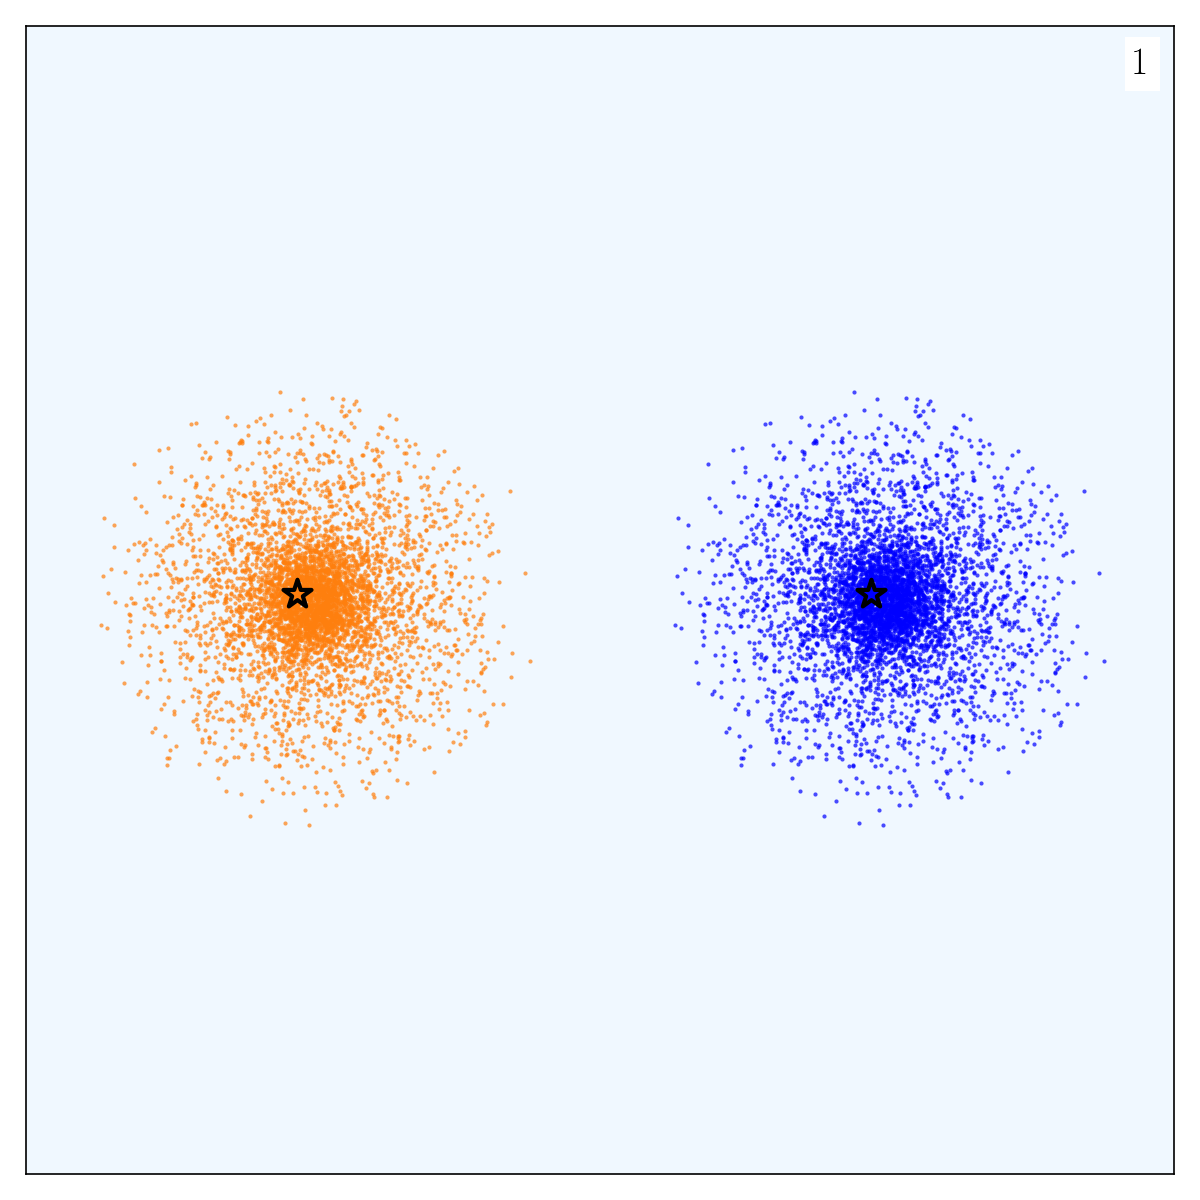
\includegraphics[width = 5.3cm]{images/jumper-demo/particleplot_00001.png}}	& 
    		{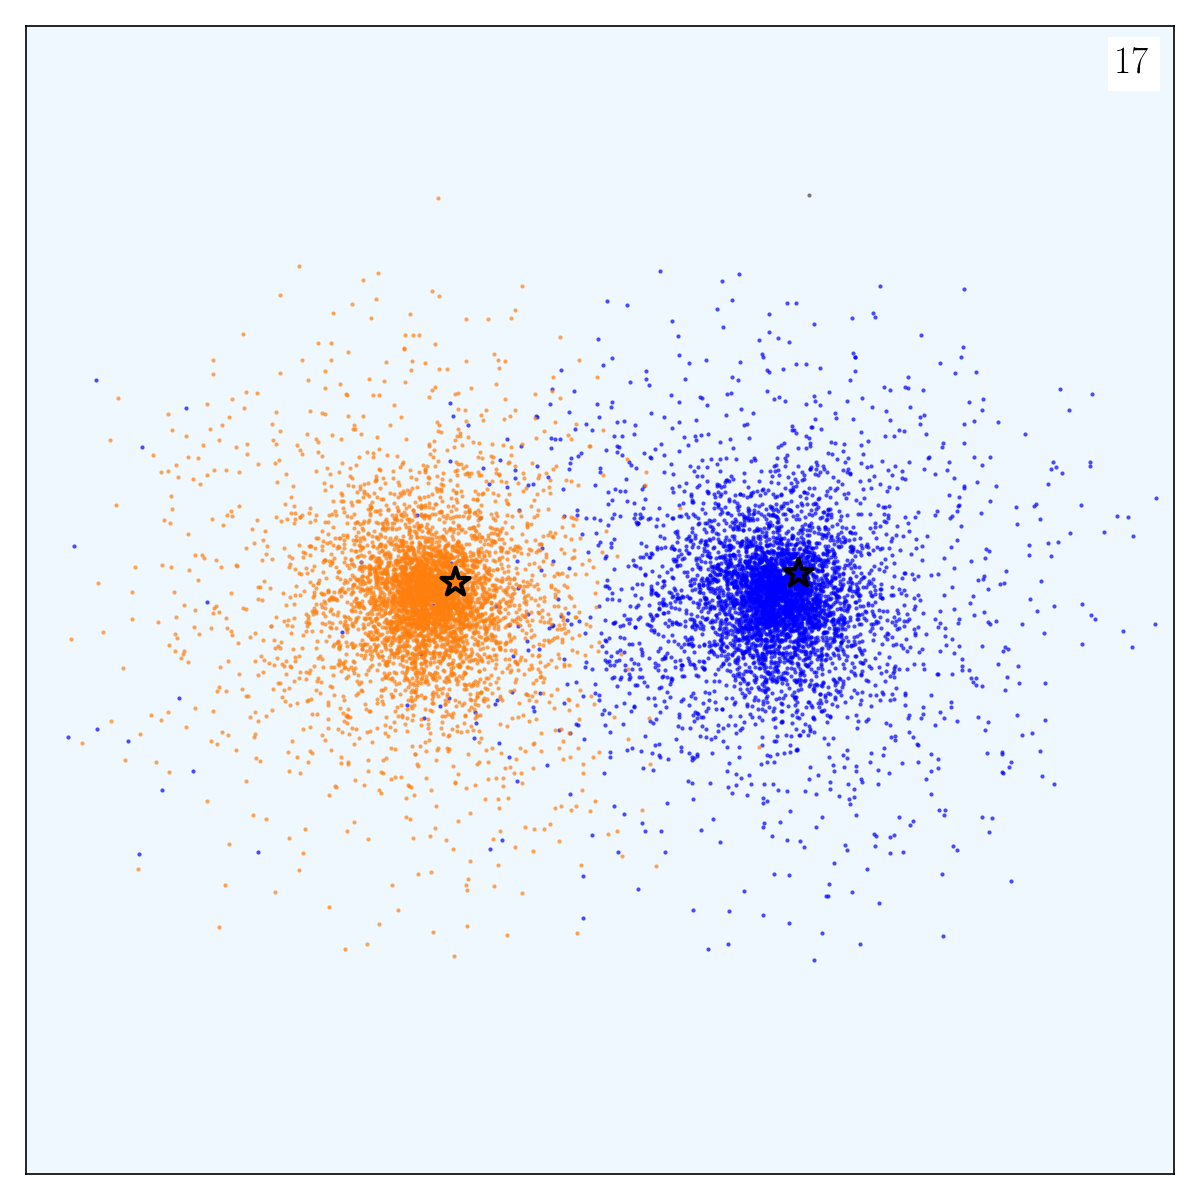
\includegraphics[width = 5.3cm]{images/jumper-demo/particleplot_00017.png}}	& 
    		{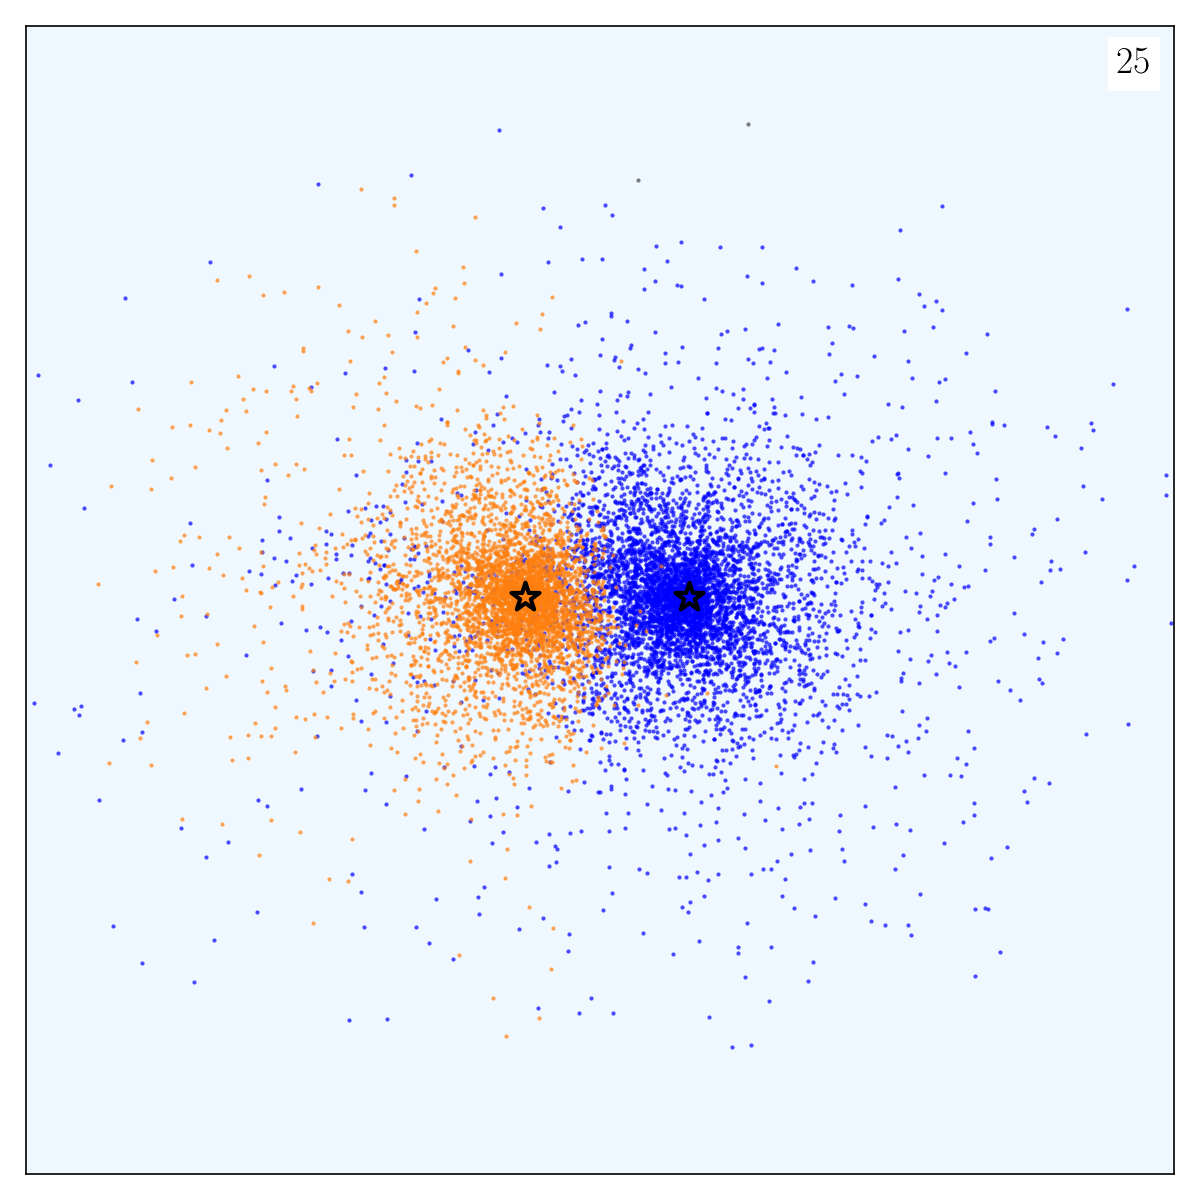
\includegraphics[width = 5.3cm]{images/jumper-demo/particleplot_00025.png}}  \\[-0.5em]
    		%
    		%
    		{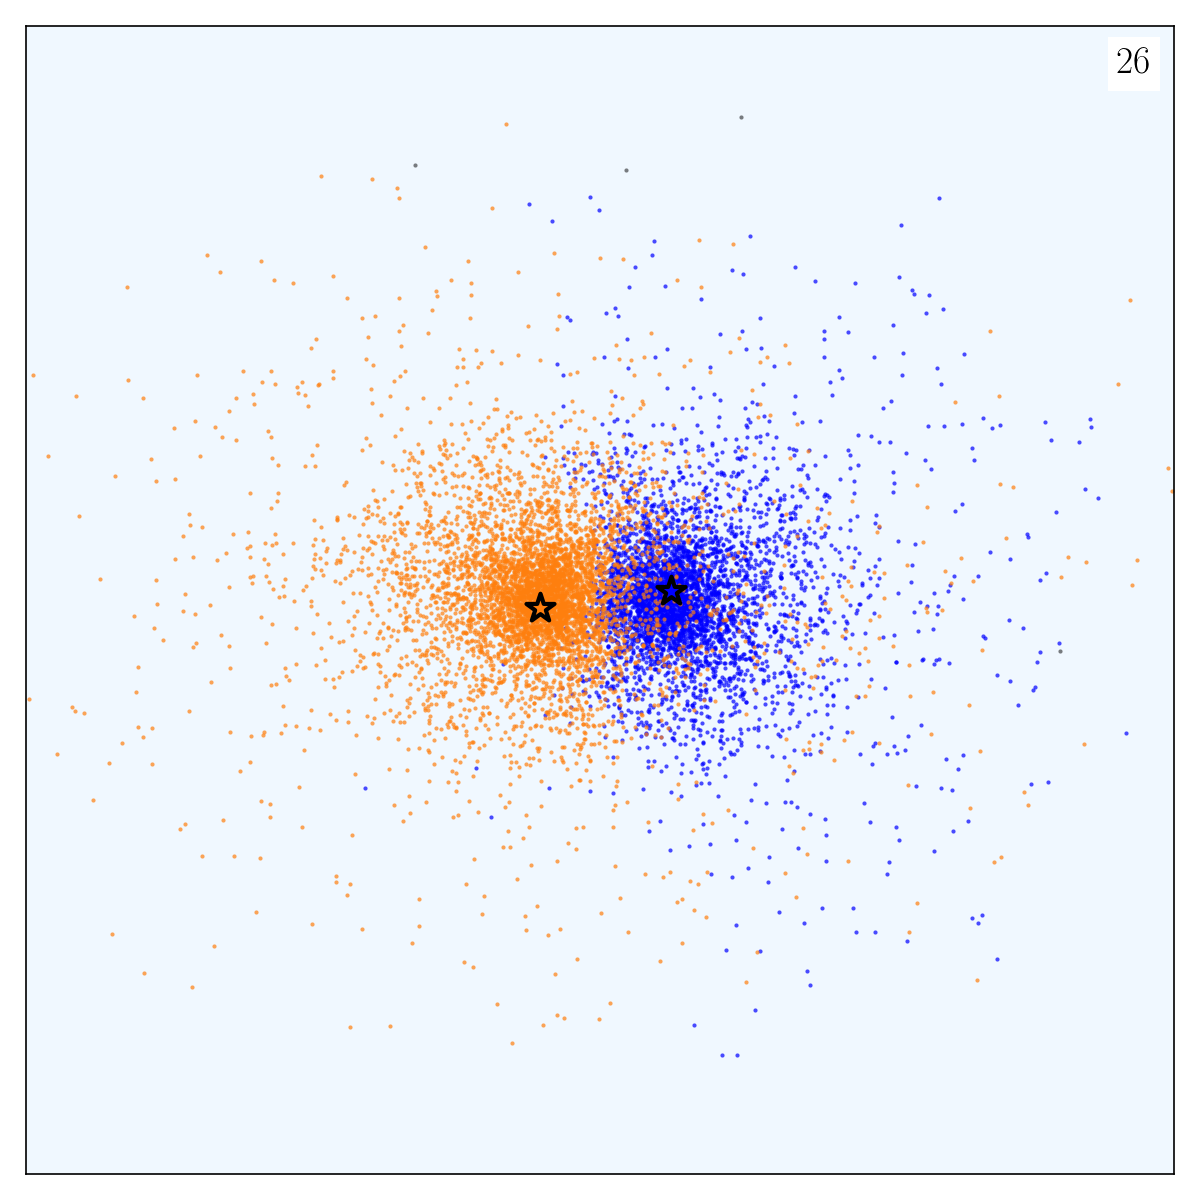
\includegraphics[width = 5.3cm]{images/jumper-demo/particleplot_00026.png}}	& 
    		{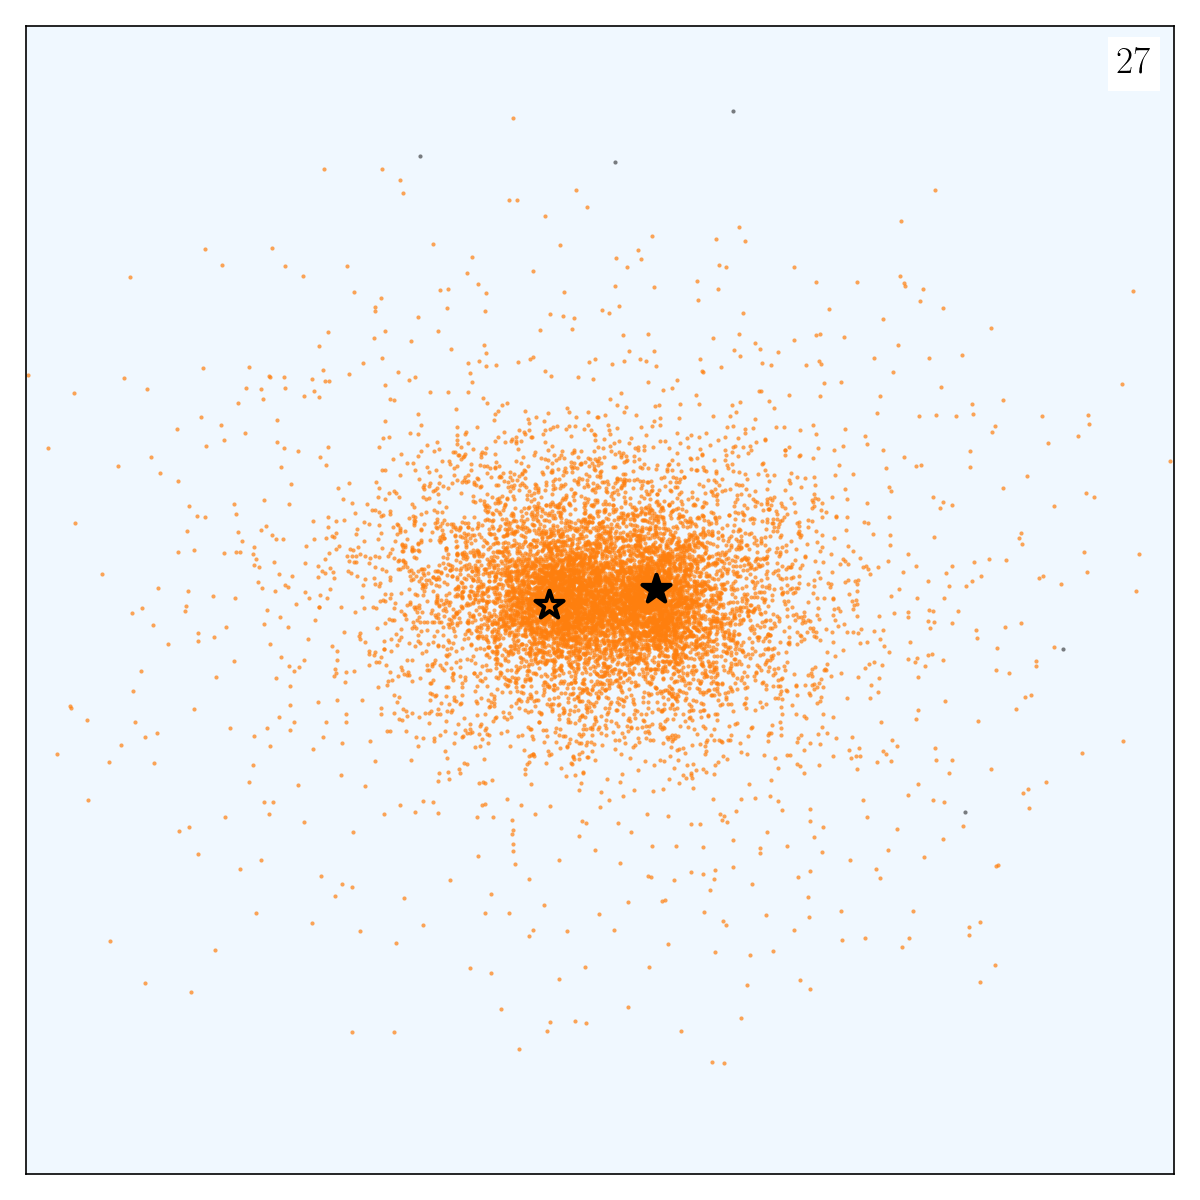
\includegraphics[width = 5.3cm]{images/jumper-demo/particleplot_00027.png}}	& 
            {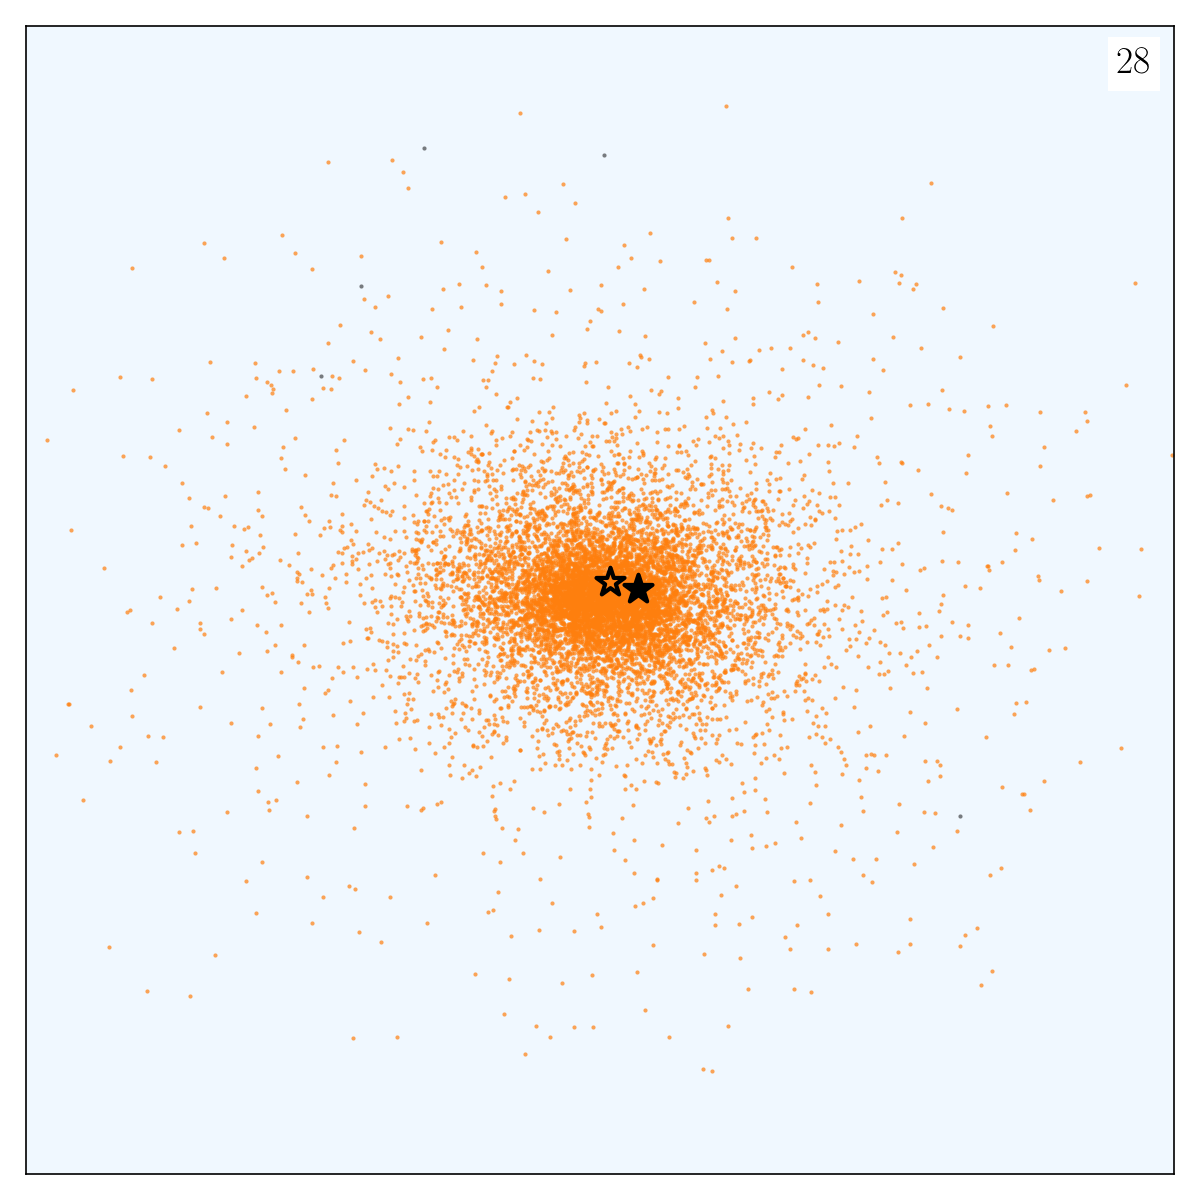
\includegraphics[width = 5.3cm]{images/jumper-demo/particleplot_00028.png}}	\\[-0.5em] 
    		%
            %
            {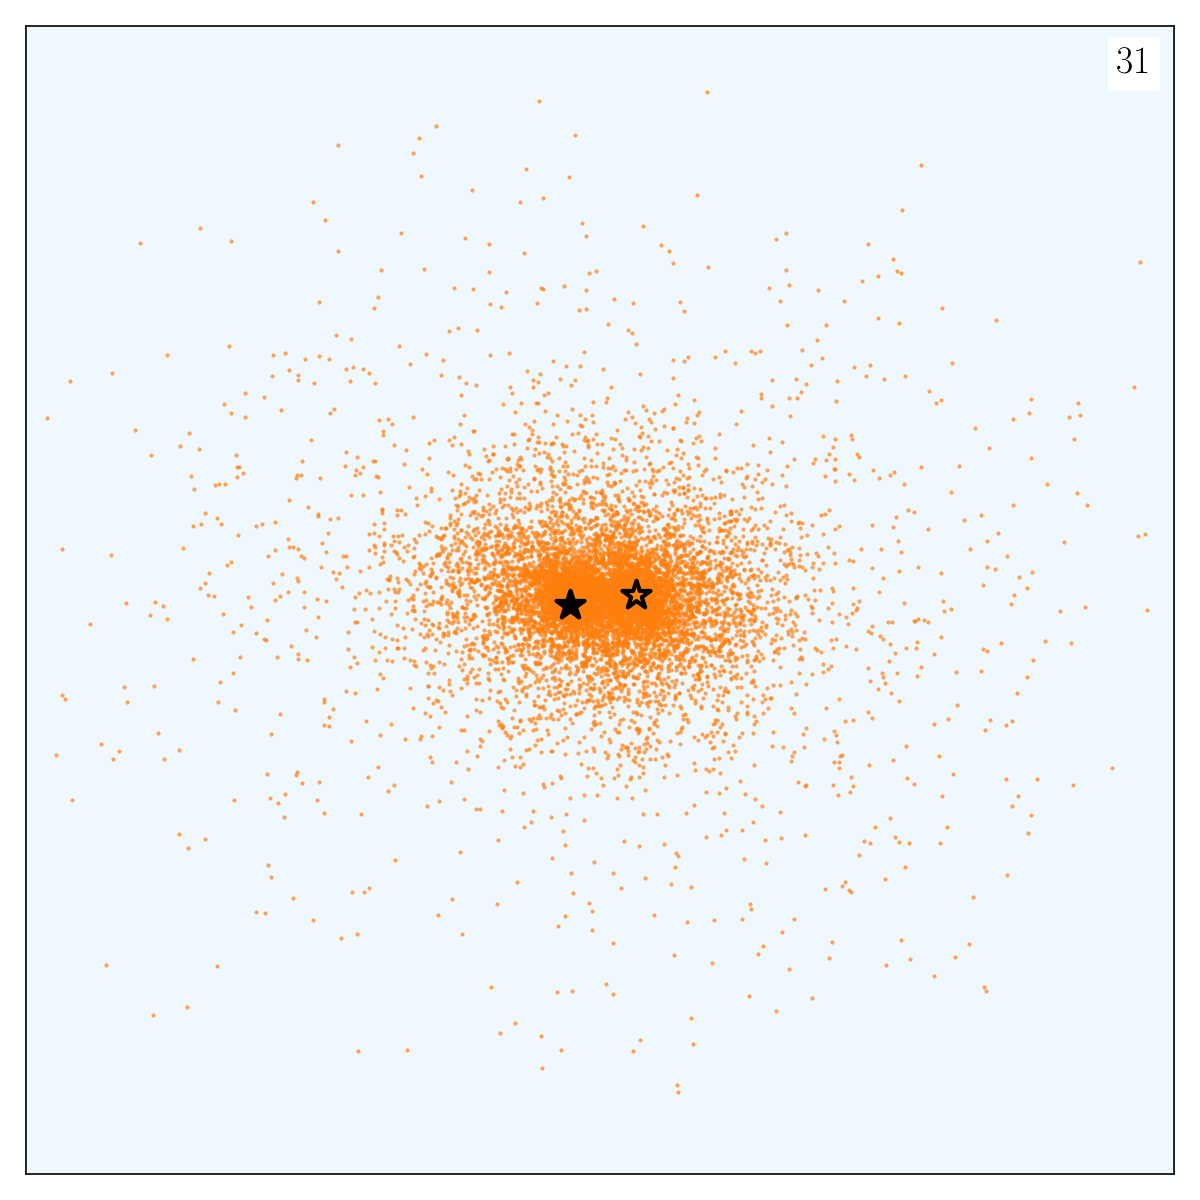
\includegraphics[width = 5.3cm]{images/jumper-demo/particleplot_00031.png}}    &
            {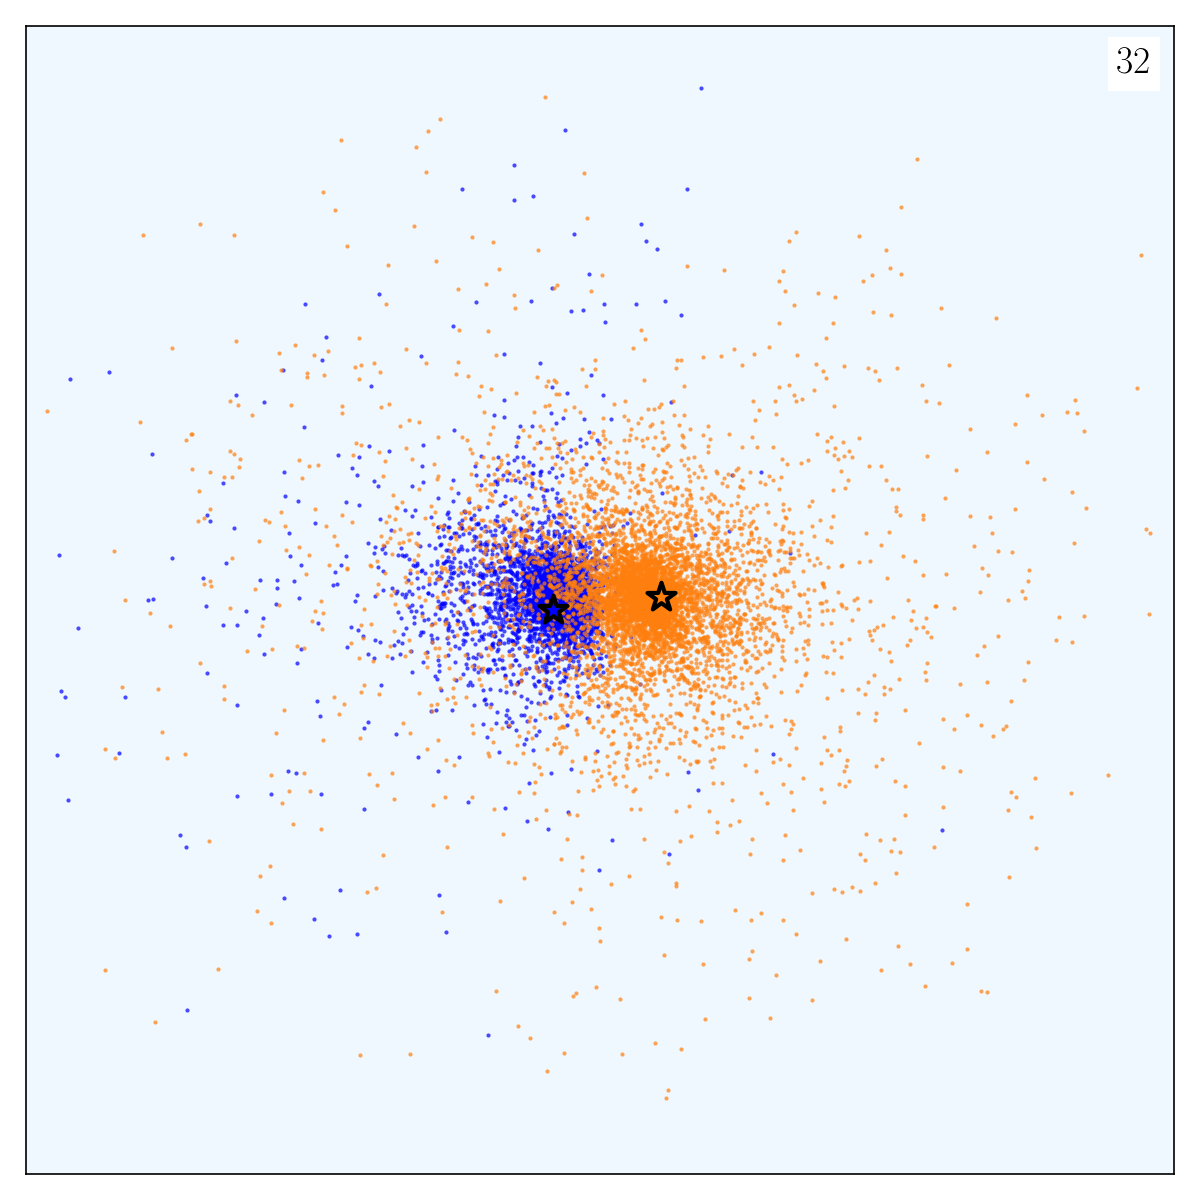
\includegraphics[width = 5.3cm]{images/jumper-demo/particleplot_00032.png}} 	&
            {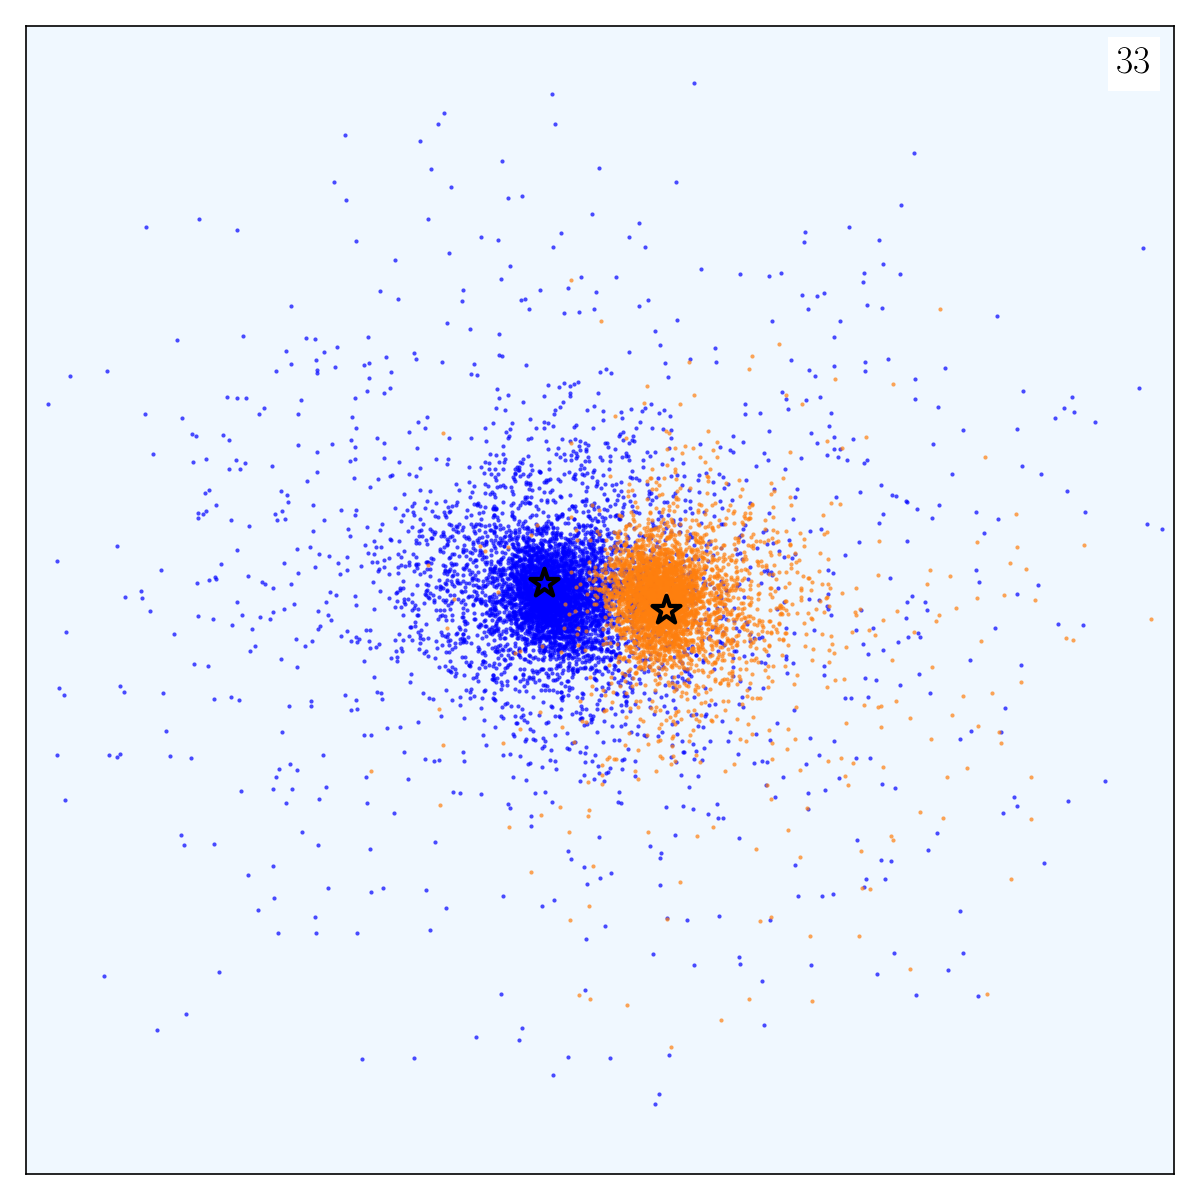
\includegraphics[width = 5.3cm]{images/jumper-demo/particleplot_00033.png}} 	\\[-0.5em]
    		%
            %
            {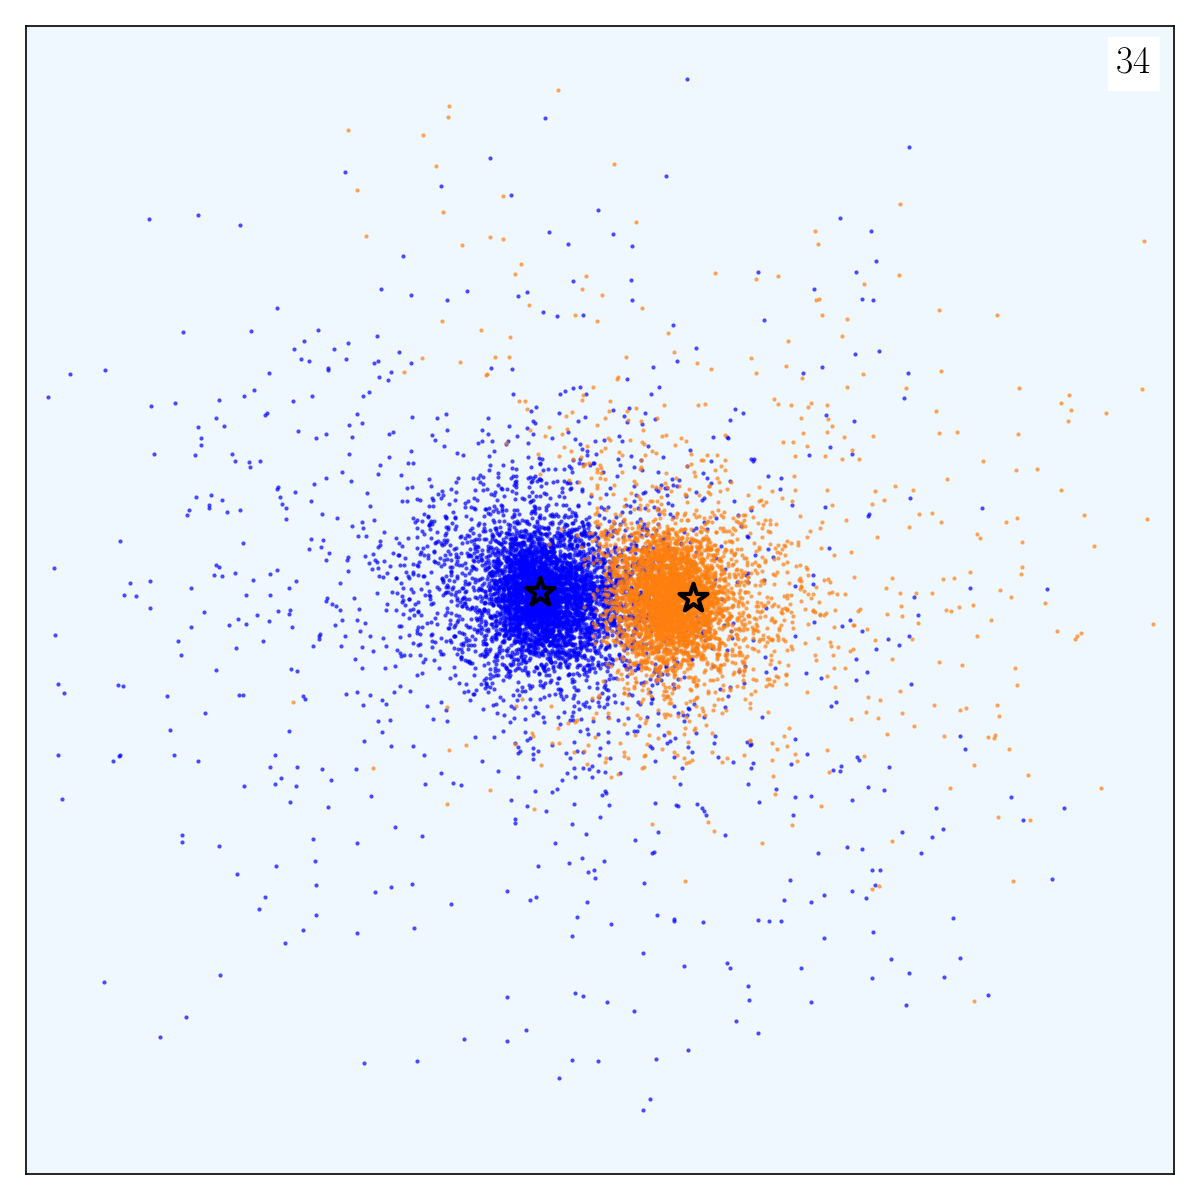
\includegraphics[width = 5.3cm]{images/jumper-demo/particleplot_00034.png}} 	& 
    		{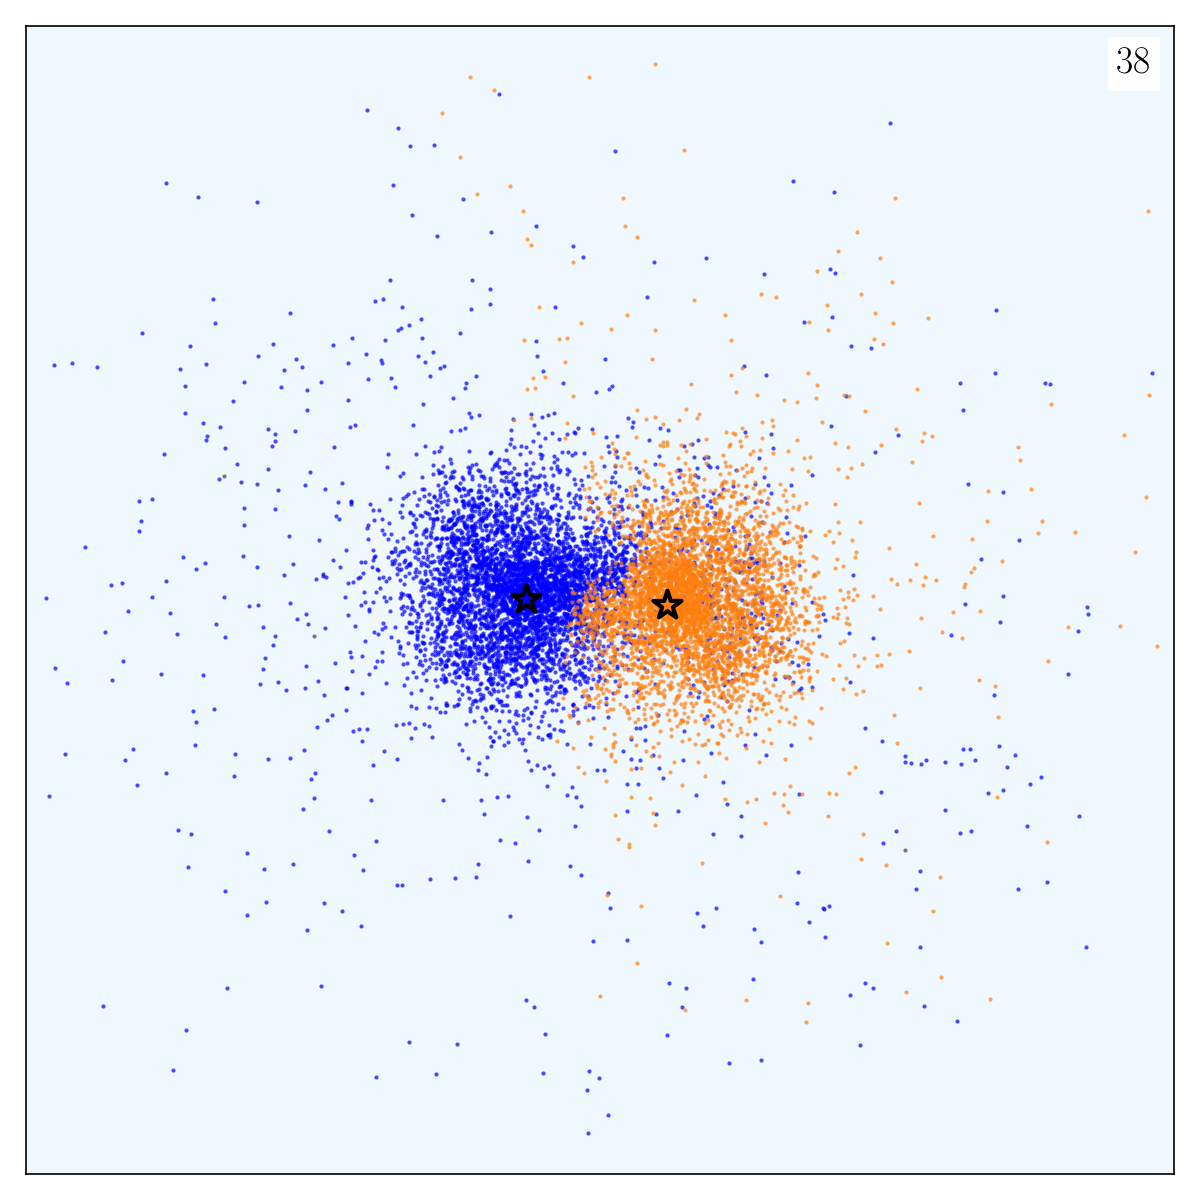
\includegraphics[width = 5.3cm]{images/jumper-demo/particleplot_00038.png}}	& 
            {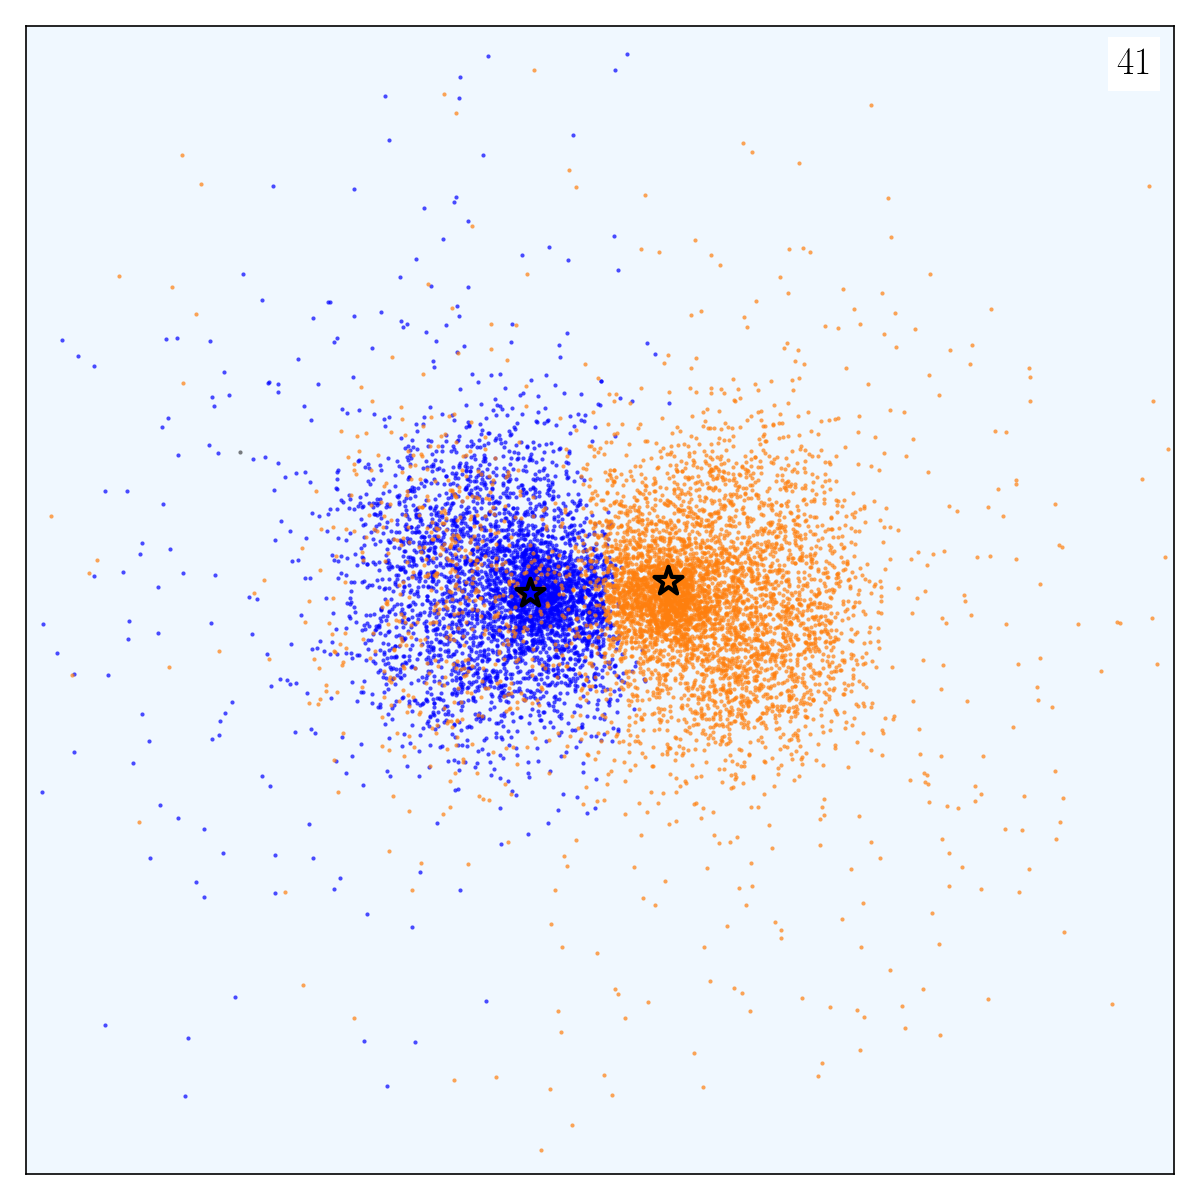
\includegraphics[width = 5.3cm]{images/jumper-demo/particleplot_00041.png}} 	\\%[-0.5em]
    		%
            %
%            {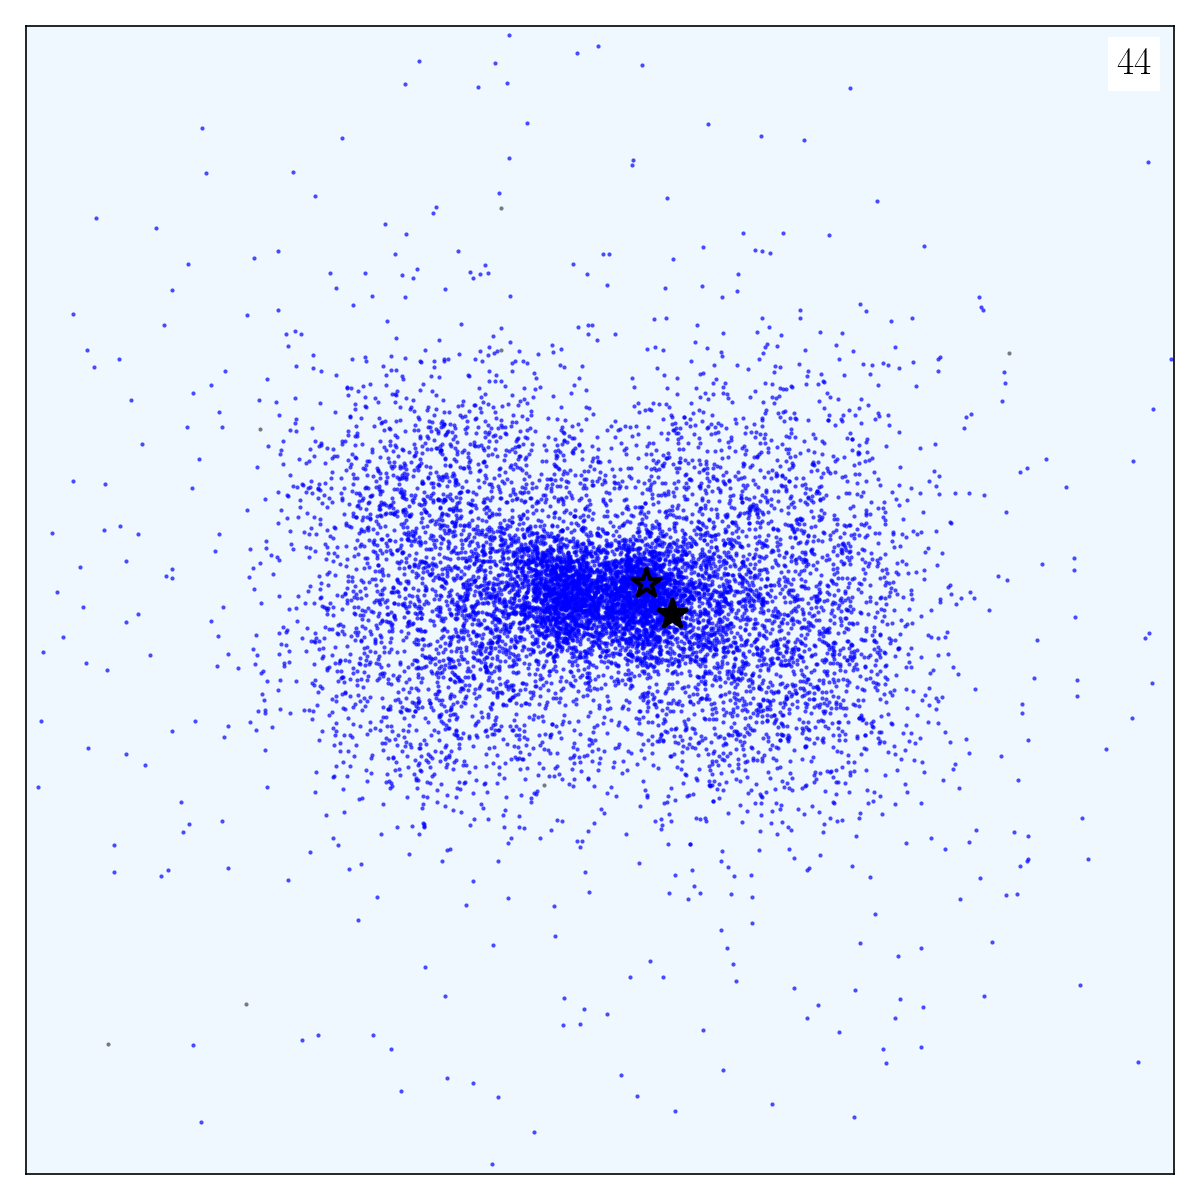
\includegraphics[width = 5.3cm]{images/jumper-demo/particleplot_00044.png}} 	& 
%    		{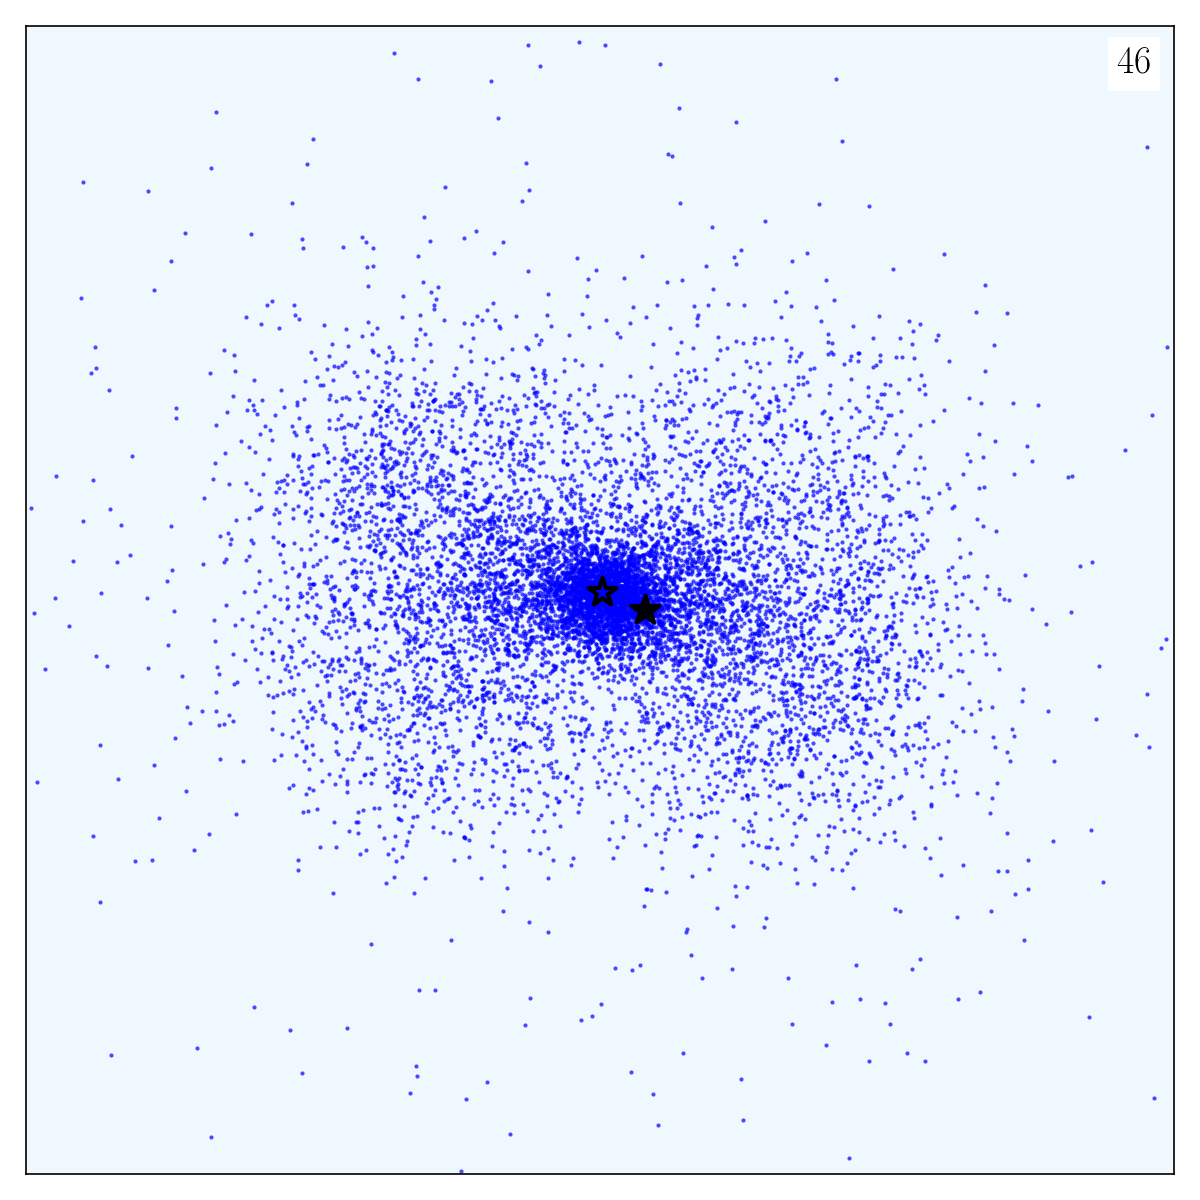
\includegraphics[width = 5.3cm]{images/jumper-demo/particleplot_00046.png}}	& 
%            {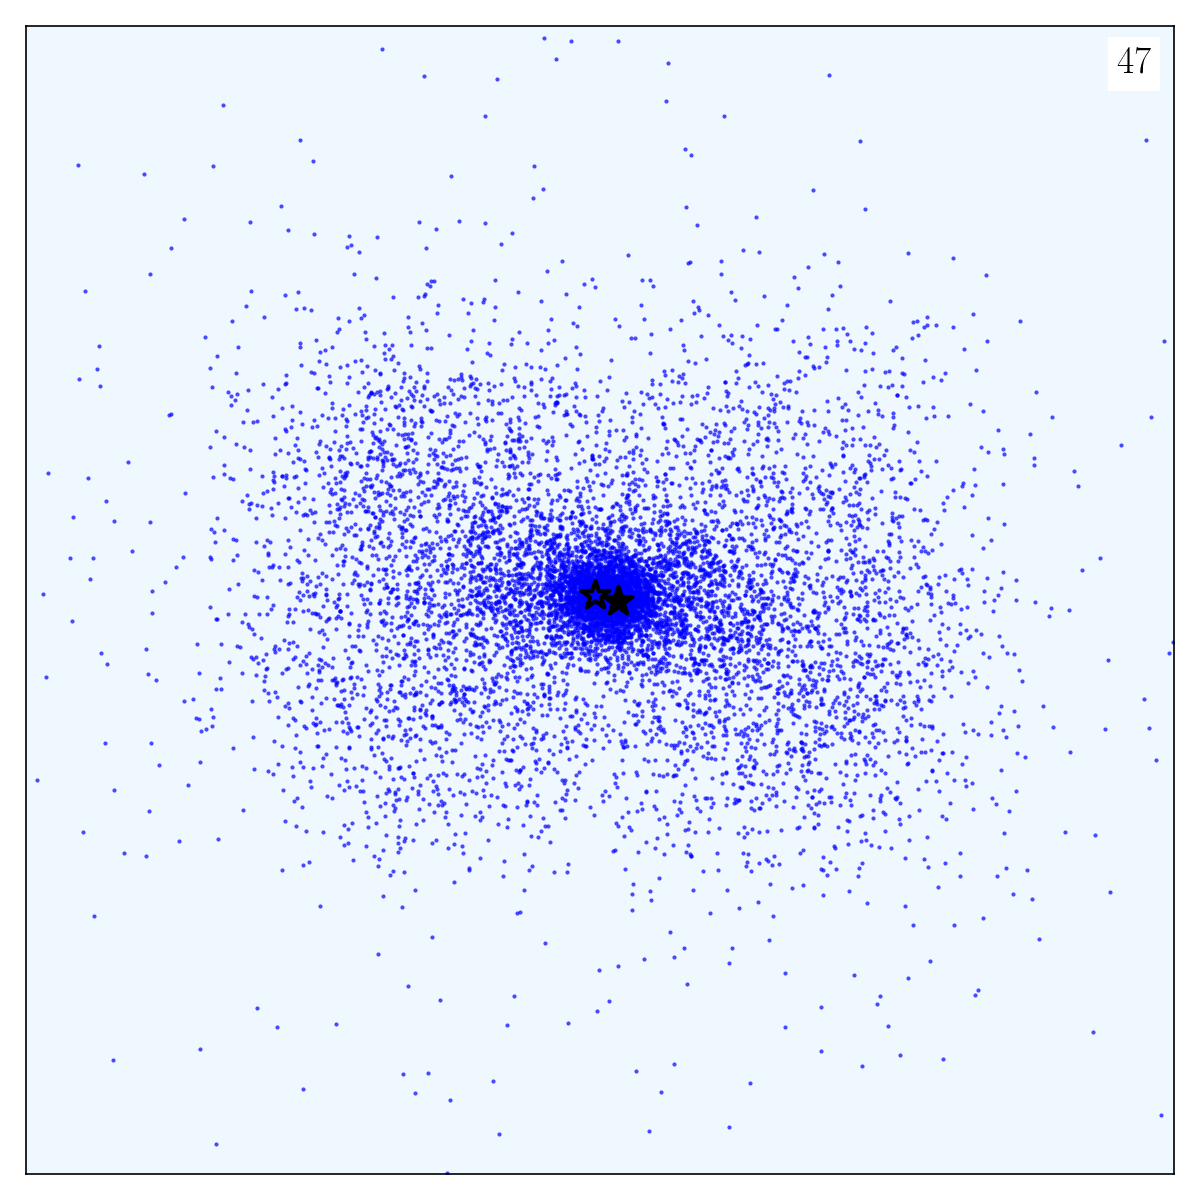
\includegraphics[width = 5.3cm]{images/jumper-demo/particleplot_00047.png}} 	& 
%            {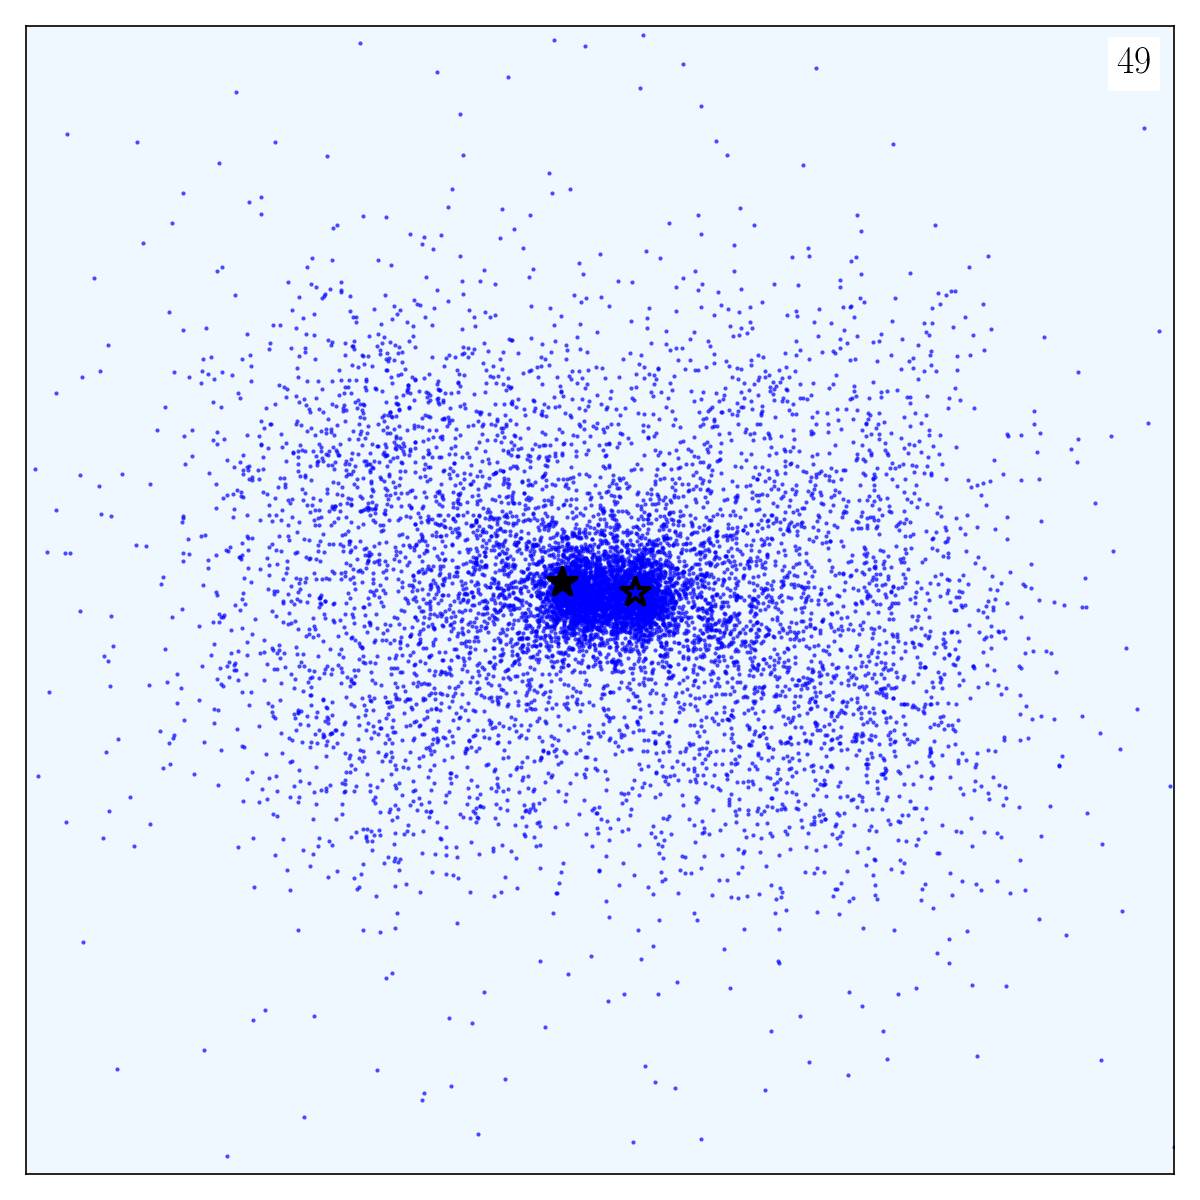
\includegraphics[width = 5.3cm]{images/jumper-demo/particleplot_00049.png}}  \\
        	\hline
    	\end{tabular}
    }
	\caption{\label{fig:jumper-demo} 
        Illustration of how haloes can seemingly merge into another one and re-appear a few snapshots later.
        The green and red particles are two initially distinct haloes that pass through each other.
        The galaxies assigned to them are marked by a star with the same colour as the particles.
        Black stars mark orphan galaxies, which have lost their unique host halo.
        The number in the upper right corner of each plot is the snapshot number that is depicted.
        In snapshots 27-31, the halo-finding algorithm didn't identify both haloes as distinct objects.
        However by tracking the red halo's orphan galaxy, it was possible to link the halo in snapshot 32 all the way back to snapshot 26.\\        
        The simulation was created using \texttt{DICE} \parencite{DICE}.
        Both haloes are identical with mass of $5\cdot 10^{10}\msol$, each containing 5000 particles and following a NFW mass profile.
        The plotted region corresponds to $400$ kpc on each side.
        }
\end{figure}




























































%\begin{sidewaysfigure}[!htbp]
%	{\renewcommand{\arraystretch}{0.1}
%		
%	\subfloat[The results of \phewon\ and \simple\ unbinding of the \ds-dataset: All particles, halo-namegiver particles only and subclumps particles only.]{
%		\begin{tabular}{|p{1cm} c c c|}
%			\hline
%			&&&\\[1em]
%													&
%			\textbf{All particles} 					&
%			\textbf{Halo-namegiver particles only} 	&
%			\textbf{Subhalo particles only} 		\\[1em]
%			%
%			%
%			\begin{sideways}{\hspace{3cm} \phewon}\end{sideways} \hspace*{-1em}%		 
%			& {\includegraphics[width = .28\textwidth]{images/dice-sub/dice-sub-plot-halo1-phew.png}} \hspace*{-1em}%
%			 & {\includegraphics[width = .28\textwidth]{images/dice-sub/dice-sub-halo-only-phew.png}} \hspace*{-1em}% 
%			 &{\includegraphics[width = .28\textwidth]{images/dice-sub/dice-sub-plot-subclumps-phew.png}} \\
%			%
%			%
%			\begin{sideways}{ \hspace{3cm}\simple\ unbinding }\end{sideways}	 \hspace*{-1em}			 &
%			{\includegraphics[width = .28\textwidth]{images/dice-sub/dice-sub-plot-halo1-nosaddle.png}} \hspace*{-1em}&
%			{\includegraphics[width = .28\textwidth]{images/dice-sub/dice-sub-halo-only-nosaddle.png}} \hspace*{-1em}&
%			{\includegraphics[width = .28\textwidth]{images/dice-sub/dice-sub-plot-subclumps-nosaddle.png}} \\
%			\hline
%		\end{tabular}
%		\label{fig:dice_sub_results_a}
%		}
%	}
%	\phantomcaption
%\end{sidewaysfigure}
%%=================================================
%%=================================================
%%=================================================
%\begin{sidewaysfigure}[!htbp]\ContinuedFloat
%	\footnotesize
%	{\renewcommand{\arraystretch}{0.1}
%	\subfloat[The results of \neigh\ and \iter\ unbinding of the \ds-dataset: All particles, halo-namegiver particles only and subclumps particles only.]{
%		\begin{tabular}{|p{1cm} c c c|}
%			\hline
%			&&&\\[1em]
%													&
%			\textbf{All particles} 					&
%			\textbf{Halo-namegiver particles only} 	&
%			\textbf{Subhalo particles only}			\\[1em]
%			%
%			%
%			\begin{sideways}{ \hspace{3cm}\neigh\ unbinding }\end{sideways}		\hspace*{-1em}		 &		
%			{\includegraphics[width = .28\textwidth]{images/dice-sub/dice-sub-plot-halo1-saddle.png}}\hspace*{-1em} &
%			{\includegraphics[width = .28\textwidth]{images/dice-sub/dice-sub-halo-only-saddle.png}}\hspace*{-1em} &
%			{\includegraphics[width = .28\textwidth]{images/dice-sub/dice-sub-plot-subclumps-saddle.png}} \\
%	%		%
%	%		%
%			\begin{sideways}{\hspace{3cm} \iter\ unbinding }\end{sideways}		\hspace*{-1em}		 &		
%			{\includegraphics[width = .28\textwidth]{images/dice-sub/dice-sub-plot-halo1-iter.png}} \hspace*{-1em}&
%			{\includegraphics[width = .28\textwidth]{images/dice-sub/dice-sub-halo-only-iter.png}} \hspace*{-1em}&
%			{\includegraphics[width = .28\textwidth]{images/dice-sub/dice-sub-plot-subclumps-iter.png}} \\
%			%
%			%
%			\hline
%		\end{tabular}
%		\label{fig:dice_sub_results_b}
%		}
%	}
%	\caption{
%	The results of different unbinding methods on the \dt-dataset.
%	}
%	\label{fig:dice_sub_results}
%\end{sidewaysfigure}
%
%









